%% Copernicus Publications Manuscript Preparation Template for LaTeX Submissions
%% ---------------------------------
%% This template should be used for copernicus.cls
%% The class file and some style files are bundled in the Copernicus Latex Package, which can be downloaded from the different journal webpages.
%% For further assistance please contact Copernicus Publications at: production@copernicus.org
%% https://publications.copernicus.org/for_authors/manuscript_preparation.html


%% Please use the following documentclass and journal abbreviations for preprints and final revised papers.

%% 2-column papers and preprints

\documentclass[amt, manuscript]{copernicus}
%\documentclass[amt]{copernicus}

%\documentclass[amt]{copernicus}




%% Journal abbreviations (please use the same for preprints and final revised papers)

%% \usepackage commands included in the copernicus.cls:
%\usepackage[german, english]{babel}
%\usepackage{tabularx}
%\usepackage{cancel}
%\usepackage{multirow}
%\usepackage{supertabular}
%\usepackage{algorithmic}
%\usepackage{algorithm}
%\usepackage{amsthm}
%\usepackage{float}
%\usepackage{subfig}
%\usepackage{rotating}

\newcommand{\todo}[1]{{\color{red} #1}}
\newcommand{\ynfcs}{y_\text{NFCS}}
\newcommand{\y}{\vec{y}}

\begin{document}

\title{Cloud correction and filtering of operational microwave humidity
  radiances with case specific uncertainty estimation}


\Author[1]{Inderpreet}{Kaur}
\Author[1]{Patrick}{Eriksson}
\Author[1]{Simon}{Pfreundschuh}

\affil[1]{Department of Space, Earth and Environment, Chalmers University of
  Technology, Gothenburg, Sweden} 

%% If authors contributed equally, please mark the respective author names with an asterisk, e.g. "\Author[2,*]{Anton}{Aman}" and "\Author[3,*]{Bradley}{Bman}" and add a further affiliation: "\affil[*]{These authors contributed equally to this work.}".


\correspondence{Inderpreet Kaur <kauri@chalmers.se>}

\runningtitle{Cloud correction with case specific uncertainty estimation}

\runningauthor{Kaur et al.}

\firstpage{1}

\maketitle


\begin{abstract}

This study presents a cloud filtering and correction method for microwave humidity radiances. The method is based on the postulation that sub-millimeter(sub-mm) frequencies can provide a basis for cloud filtering/correction of data measured around 183\,GHz. A quantile regression(QRNN) based approach is formulated to estimate the posterior distributions of noise free clear sky (NFCS) radiances. QRNNs are trained to correct the cloud impact for each 183\,GHz channel using measurements from the target channel and available sub-mm channels. The approach is demonstrated by application to Ice Cloud Imager(ICI) and MicroWave Imager (MWI). As a special case, applicability to smaller satellite missions like Arctic Weather Satellite (AWS), with fewer sub-mm channels, is also evaluated. The performance of QRNN based cloud filtering is also investigated. The results are compared against the NFCS simulations.

Pure-filtering approach is only partially successful in removing the cloud contamination. Though most of the cases with high cloud impact are drawn out, cases with low cloud impact are falsely classified as cloudy. This shortcoming is unacceptable in retrieval and assimilation applications and reinforces the necessity for cloud correction. The results from cloud correction show that QRNN is successful in alleviating the cloud contamination to a large extent. Few cases with residual cloud impact deteriorate the performance but filtering out such cases results in error distributions which are symmetric and have low bias and standard deviation. In some cases, the combination of 183\,GHz and sub-mm channels also results in a lower variability than noise. Another advantage of using QRNN is that predicted quantiles can be employed to quantify the case-specific uncertainty estimates.  The results show that QRNN is successful in representing the uncertainty for most of scenes individually. Despite individual variations for each channel, it is observed that uncertainty consistently increases with the error in the performance. 

The results show that it can be highly recommended to use all available sub-mm frequencies to estimate the NFCS values of radiances/brightness temperatures. The strategy works well even when only one of the higher frequencies is available. This study uses simulated data, but we can expect to obtain similar performance when data from the new sensors will be available. 
     
\end{abstract}


\copyrightstatement{TEXT}


\introduction
%
Satellite observations of humidity inside the troposphere are mainly performed
by downward-looking sensors. Among this class of observations, the frequency
range around 183\,GHz has a special position. Water vapour has a noticeable
transition at 22\,GHz, but it is relatively weak and only column values can be
derived \citep[e.g.][]{schluessel1990atmospheric} for the observation geometry
of concern. The first transition in the microwave region that can be used to
derive altitude information, i.e.\ can be used for ``sounding'', is the one at
183.31\,GHz \citep{kakar1983retrieval,wang1983profiling}. On the other hand, at
infrared wavelengths a high number of water vapour transitions are found,
including some of high strength. As a consequence, infrared sounders can
provide humidity profiles with high precision and good vertical resolution, but
with strong limitations imposed by clouds. To be able to also sense humidity
inside and below clouds, weather satellites are since some time equipped with
channels around 183\,GHz. Today such channels are part of several sensors, such
as ATMS (Advanced Technology Microwave Sounder, \citet{weng2012introduction}).

Precipitation and most dense clouds, particularly if found at high altitude, can
still affect measured radiances around 183\,GHz
\citep[e.g.][]{bennartz2003sensitivity}. As the impact from the hydrometeors
then is dominated by scattering, the complexity of the analysis of the data
increases dramatically and there exists a need to identify the problematic
cases. This is normally denoted as cloud filtering, to obtain data of ``clear
sky'' character. Such filtering has been applied to derive climate records
\citep{lang2020new} and is essential in studies of the agreement between
observations and simulations \citep{brogniez2016review} as well as 
comparing observations of different instruments to validate their calibration
\citep{john2013assessment,moradi:retri:15,berg2016intercalibration}. A commonly
used cloud filtering methods for these applications is the one of
\citet{buehler:aclou:07}. This method is based on the 183\,GHz data alone,
involving rules on the brightness temperatures differences between channels. An
older version is \citet{burns1997effects}.

The main motivation for introducing 183\,GHz channels in operational sensors is
numerical weather prediction (NWP). Usage of passive microwave data by
``all-sky'' assimilation in global NWP is growing in \citep{geer2017growing},
but 183\,GHz data are still mainly used in a clear sky fashion
\citep{geer2018all}. The later is particularly true in NWP of regional scope
\citep{gustafsson2018survey}, all-sky assimilation of 183\,GHz at many national
weather agencies will likely not be reached in many years. Anyhow, the cloud
filtering applied differs between NWP centres. One approach is to make use of a
``scattering index'' \citep{bennartz2002precipitation}, based on the
observations alone. Today, likely more common is to use ``observation minus
background'' (O-B), where the forecast model is used to obtain an estimate of
the expected clear-sky value and the observation is rejected if the deviation
exceeds some threshold (???). In both cases, the filtering typically involves
observations around 89 and/or 150\,GHz.

Despite the broad usage these filtering methods have some drawbacks. For
183\,GHz, the impact of hydrometeors systematically causes a decrease in the
observed radiance (maybe with exceptions at extremely dry conditions), see
e.g.\ \citet{barlakas:three:20} and below. This means that if any cloud
contamination is missed by the filtering this will cause a negative bias in
mean radiance, compared to the true clear-sky mean. This bias will translate to
a bias in humidity after the retrieval or assimilation. The alternative is to
apply a very strict filtering, but this will result in that a high fraction of
actually clear-sky values will be rejected, i.e.\ an important loss of useful
data.

The filtering is normally done in a ``one for all'' manner, i.e.\ all 183\,GHz
channels are either kept or rejected, while, as the channels differ in their
altitude coverage, there could be cloud impact in some channels and still the
others can be considered as clear-sky. To allow a channel specific filtering,
data likely need to be combined in a more complex manner than simple
differences, but it is unclear what type of regression that would be best. This
points towards applying machine learning, as used by e.g.\
\citet{favrichon2019detecting}.

A maybe less obvious problem is the uncertainty to assign to the filtered
values. To our best knowledge, so far only estimates of mean and worst case
errors have been provided. Some cases with relatively high cloud impact will
likely be missed, while most cases are clear sky from start. As the remaining
cloudy cases can cause significant biases, the likely solution is to apply a
quite conservative (high) error estimate. However, this will unnecessary
downgrade the value of the truly clear sky cases and the observations are used
in a non-optimal manner.

We are here approaching cloud filtering task from a new angle. The basic idea
is to derive an estimate of the corresponding noise-free clear-sky (NFCS) value
(i.e.\ the radiance that would have been measured in absence of noise and
hydrometeors). This is done for each channel separately, only using
measurements (no ``background'' data involved). Not only a best estimate is
provided, but also a case specific uncertainty.

This information can be used as a pure filter, by rejecting data where the
correction exceeds some threshold value. This threshold value should be
relatively low, to not introduce a bias in filtered dataset. However, even
better is to replace the original value with the predicted NFCS value when
forming the clear-sky dataset. This approach we denote as cloud correction. It
is shown below that a basically bias free cloud correction can be obtained.
This feature removes the need of threshold value, as long as the retrieval or
assimilation system can incorporate the uncertainty of the corrected value. As
also will be shown, the uncertainty for originally clear sky data is determined
by noise, but the uncertainty increases with magnitude of correction.
Accordingly, the cloud correction approach allows that the full weight of
clear-sky data can be preserved.

The estimation of NFCS values makes use of a special type of machine learning,
denoted as Quantile Regression Neural Network (QRNN,
\citet{pfreundschuh:aneur:18}). Unlike standard usage of machine learning where
only some kind of best estimate is provided, QRNN works in a Bayesian fashion
and instead gives a description of the posterior uncertainty. More precisely,
QRNN outputs an user specified set of percentiles that gives a discrete
description posterior distribution, that can be process to derive e.g.\ the
expectation value.

The approach is demonstrated on a combination of 183\,GHz channels (following
\citet{buehler:aclou:07}), but we mainly explore the cloud correction (of
183\,GHz data) that will be possible when sub-millimetre data will be at hand
in some years. This wavelength region will be introduced by the Ice Cloud
Imager (ICI, \citet{eriksson:towar:20}), but likely also be included in several
smaller missions (such as AWS, presented below). \todo{Explain what sub-mm can
  do}.

The focus on ICI is motivated by several reasons. The true potential of the
QRNN cloud correction approach is likely not revealed if tested on existing
data and applying ICI data for cloud filtering has not earlier been discussed.
It is also argued that the cloud correction makes it possible to make good use
of ICI data already in clear-sky assimilation, a fact that should speed up the
use of this novel data source.



\section{Data and methods}
%
\subsection{Satellite Instruments}
\subsubsection{Ice Cloud Imager}
%
%t
\begin{table*}[t]	
	\caption{Specifications of ICI and MWI channels relevant to this study.}
	\label{tab:ICI_MWI_channels}
	\begin{tabular}{lrrr}
		\tophline
		Channel & Frequency 	& Bandwidth  	&NE$\Delta$T	\\
				& [GHz]			& [MHz]			& [K]			\\
		\middlehline
		I1V&	183.31$\pm$7.00    & 2000 			& 0.8 		\\
		I2V&	183.31$\pm$3.40    & 1500 			& 0.8 		\\
		I3V&	183.31$\pm$2.00    & 1500			& 0.8 		\\
		I5V&	325.15$\pm$9.50    & 3000			& 1.2 		\\
		I6V&	325.15$\pm$3.50    & 2400			& 1.3 		\\
		I6V&	325.15$\pm$1.50    & 1600			& 1.5 		\\
		I8V&	448.00$\pm$7.20    & 3000			& 1.4 		\\
		I9V&	448.00$\pm$3.00    & 2000			& 1.6 		\\
		I10V&	448.00$\pm$1.40    & 1200			& 2.0 		\\
		I11V&	664.00$\pm$4.20    & \phantom{0}500	& 1.6 		\\
		I11H&	664.00$\pm$4.20    & \phantom{0}500 & 1.6 		\\		
		\bottomhline
	\end{tabular}
	\begin{tabular}{lrrr}
		\tophline
		Channel & Frequency 	& Bandwidth  	&NE$\Delta$T	n\\
				& [GHz]			& [MHz]			& [K]			\\
		\middlehline
		MWI-14&	183.31$\pm$7.00    & 2000 			& 1.3 		\\
		MWI-15&	183.31$\pm$6.10    & 1500			& 1.2 		\\
		MWI-16&	183.31$\pm$4.90    & 1500			& 1.2 		\\
		MWI-17&	183.31$\pm$3.40    & 1500			& 1.2 		\\
		MWI-18&	183.31$\pm$2.00    & 1500			& 1.3 		\\	
		\bottomhline
	\end{tabular}

	\belowtable{} % Table Footnotes
\end{table*}

Ice Cloud Imager (ICI) is a new instrument on board EPS-SG(EUMETSAT Polar System - Second Generation) satellite Metop-SG. Metop-SG is scheduled for launch in 2023, and it will make ICI the first operational sensor observing Earth using sub-millimeter(sub-mm) wavelengths. ICI is a conically scanning radiometer that will measure 13 frequencies from 183 GHz up to 664 GHz. The main objective of ICI is to use high frequency channels for measuring ice cloud properties and improve the representation of ice clouds in regional and global Numerical Weather Prediction(NWP) models. ICI consists of channels receiving frequencies around 183.31\,GHz, 325.15\,GHz and 448.00\,GHz, measuring vertical polarization. While other channels around frequencies 243.20\,GHz and 664.00\,GHz are ``window channels'' and measure both vertical and horizontal polarization. The instrument will observe earth from a mean altitude of 832\,Km with sensor viewing angle 44.767$^\circ$(measured from nadir). For all the channels, the mean footprint size is about 15\,Km, but the exact geo-location of samples differs. Therefore a simultaneous utilization of data from different channels requires remapping to a common footprint \citep{eriksson:towar:20}.

For this study, we conducted the forward simulations at frequencies: 183.31\,GHz, 325.15\,GHz, 448.00\,GHz and 664.00\,GHz(See Table~\ref{tab:ICI_MWI_channels}). For brevity, we assumed that all simulations were mapped to a common footprint.

\subsubsection{MicroWave Imager}
%
\label{mwi_channels}
In addition to ICI, the Metop-SG will also have Microwave Imager(MWI) on board. MWI is a conically scanning radiometer and will measure frequencies from 18 GHz up to 183\,GHz \todo{add ref}. All channels up to 89 GHz will receive both horizontal and vertical polarisation, while other frequencies will receive only vertical polarisation. A short summary of the MWI channels used in the study is provided in Table~\ref{tab:ICI_MWI_channels}. MWI also has three  183\,GHz frequencies in common with ICI. The overlapping frequencies shall allow cross-calibration between the two instruments, and provide microwave measurements from 18\,GHz to 664\,GHz on a common scale. The main objective of MWI is to provide data continuity to the existing microwave imager measurements for cloud and precipitation and support regional and global NWP models.

For this study, forward simulations at frequencies around 183.31\,GHz were performed. When ICI and MWI simulations were used together, MWI channels were assumed to be mapped to ICI footprint and resolution. Remapping reduces the noise in MWI from 1.2\,K at 10\,Km resolution to 0.8\,K at 15\,Km resolution.  

\subsubsection{Artic Weather Satellite}
%
\begin{table}[t]
	\caption{Specifications of AWS channels relevant to this study.}
	\label{tab:specifications_AWS}	
	\begin{tabular}{lrrr}
		\tophline
		Channel & Frequency 	& Bandwidth & NE$\Delta$T \\
				& [GHz]			& [MHz]		& [K]		\\
		\middlehline
		AWS-32	&	176.311    & 2000	&		\\
		AWS-33	&	178.811    & 2000 	&	\\
		AWS-34	&	180.311    & 1000 	&	\\
		AWS-35	&	181.511    & 1000 	&	 \\
		AWS-36	&	182.311    & \phantom{0}500  &	 \\
		AWS-41  & 325.15$\pm$6.60    & 2800 	 &0.60\\
		AWS-42  & 325.15$\pm$4.10    & 1800    &0.75	\\
		AWS-43  & 325.15$\pm$2.40    & 1200    &0.92\\
		AWS-44  & 325.15$\pm$1.20    & \phantom{0}800  &1.12  \\
		\bottomhline
	\end{tabular}
	\belowtable{} % Table Footnotes
\end{table}
The Arctic Weather Satellite (AWS) is a small satellite mission approved as ESA
Earth Watch Programme Element. It is a small platform carrying a single across-track scanning microwave radiometer. It is planned as a small but cost-effective platform, which can supplement the information from other polar orbiting satellites. The first prototype mission is expected to be delivered around 2023. The main objective of AWS will be to improve the representation of Artic and sub-Arctic weather in NWP models and improve the global weather forecasts. AWS will will have channels receiving frequencies around 89.00\,GHz, 165.5\,GHz, 183.31\,GHz, 229.00\,GHz and 325.15\,GHz. For a detailed description of the AWS channels see \citet{eriksson2020study}. 

In this study, forward simulations at frequencies 183.31\,GHz and 325.15\,GHz were conducted. A brief summary of these channels is provided in Table~\ref{tab:specifications_AWS}.

\subsubsection{Cloud Profiling Radar}
%
Cloud Profiling Radar(CPR) is the main instrument on sun-synchronous polar orbit satellite CloudSat (Cloud Satellite) \citep{Stephens2002cloudsat}. It was launched in 2006 and is part of the A-train constellation of four earth observation satellites. CPR is a nadir looking radar operating at 94.05\,GHz and measures the cloud backscatter as a function of distance from the radar, to provide vertical profiles of clouds and precipitation.

In this study, CloudSat profiles were used only to perform the forward simulations for ICI, MWI and AWS. 

\subsection{Simulations}
\label{sec:arts_simulations}
%
\subsubsection{Input data}
%
Cloudsat profiles during August 2015 were randomly selected for forward simulations. The input data were restricted between $60^{\degree}$S to $60^{\degree}$N, and surface is below 500\,m. Both clear-sky and all-sky scenarios were simulated, and no differentiation was made between the observations over ocean/sea and land. 
\subsubsection{Simulation setup}
%
**** Some parts copied directly from AWS report *****

The absorption model takes into account the effect from nitrogen
\citep{pwr:93}, oxygen \citep{pwr:93} and water vapour
\citep{ellison2007permittivity}. LWC is taken from ERA-Interim and is assumed
to be totally absorbing. In the mapping of CloudSat reflectivities to RWC and
IWC a total separation between liquid and ice phase is assumed. All scattering
hydrometeors at temperatures above 0$^\circ$C are assumed to be rain, and all
below 0$^\circ$C are assumed to be ice hydrometeors. For RWC the particle size
distribution of \citet{abel2012improved} is applied. The PSD of IWC follows the
basic formulation applied in DARDAR (\verb
http://www.icare.univ-lille1.fr/projects/dardar), using latest parameter
values (i.e.\ $\alpha$ and $\beta$) as given by \citet{cazenave2019evolution}.
This PSD can be considered as a ``two moment'' scheme, but is here applied in
a one moment manner by setting $N_0^*$ (as a function of temperature)
following Table~5 of \citet{delanoe2014normalized}, and letting the radar
reflectivity set the remaining moment. Single scattering data are taken from
\citet{eriksson:agene:18}. For ice hydrometeors, three habits are applied:
Perpendicular 3-bullet rosette, Large plate aggregate and Large column
aggregate. In the last two cases, the aggregates are complemented with single
crystal data to also cover smaller sizes. These data describe particles
assumed to have a totally random orientation. To apply oriented particles is
much more computationally costly and could not be accommodated inside the
study. The land emissivity was taken from TELSEM \citep{aires2011tool} and the
Ocean/water from TESSEM \citep{prigent2017sea}. For each atmopsheric case,
both ''clear-sky'' and ``all-sky'' calculations were performed. In the former,
all impact of all hydrometeors were set to zero, while in the latter, IWC and
RWC derived from CloudSat reflectivities and LWC from ERA-Interim were taken
into account. Both sets of calculations were made by ARTS's interface to the
RT4 solver \citep{evans1995microwavec}. To avoid a possible bias between
clear-sky and all-sky for insignificant hydrometeor contents, the same
``scattering solver'' was used for both calculations. The first two elements
of the Stokes vector were calculated.

\subsubsection{Produced dataset}
%
Using the simulation setup described in previous section,  
220\,000 cases for each ICI and MWI frequency were simulated. For both instruments, the channel frequencies were simulated directly. For AWS, 140\,000 cases were simulated. Forward simulations were performed for 21 monochromatic frequencies. These frequencies were interpolated to a finer grid to get the AWS channel brightness temperatures. All AWS sensor viewing angles (from $0^\circ$ to $45^\circ$) were simulated, but the results described in this study are based on nadir viewing angle. 

ARTS simulations are noise free, so to incorporate the measurement uncertainties, whenever needed, gaussian noise was added to according to the channel NE$\Delta$T (Table~\ref{tab:ICI_MWI_channels},Table~\ref{tab:specifications_AWS}). For cases where MWI and ICI simulations were assumed to be remapped to a common footprint, the NE$\Delta$T for corresponding to ICI channels was used (See Sect.~\ref{mwi_channels}).

The noise free simulations were divided into training and testing datasets. Out of the 220\,000 simulations for ICI and MWI each, 175\,000 cases were randomly picked to form the training set. The rest were used for testing. A smaller database was selected for AWS. 120\,000 simulations were used for training and the remaining were used for testing.

\subsection{Quantile regression neural networks}
%
The task that we aim to solve in this study is to predict the NFCS brightness
temperature $\ynfcs$ at a given $187\unit{GHz}$ channel from a vector of
cloud-contaminated observations $\y$. Since the information-content of the
cloud-contaminated observations is certainly too low to solve this problem
exactly, a probabilistic formulation is appropriate here. The aim thus becomes
to predict the conditional distribution $p(\ynfcs | \y)$ of the NFCS brightness
temperatures $\ynfcs$ given the cloud-contaminated observations $\y$.

As has been shown in \citet{pfreundschuh:aneur:18}, quantile regression neural
networks (QRNN) can be used to solve these type of problems. Instead of a point
prediction, as it is typically performed in regression problems, QRNNs learn to
predict a vector of quantiles, which can be used to approximate the distribution
of the predicted quantity conditional on the network inputs. Using QRNNs to
perform probabilistic cloud correction thus not only allows deriving an estimate
for $\ynfcs$ but also for the error of the corrected observations.

For this application, the predicted percentiles are chosen to be
$0.2\%, 3\%, 16\%, 50\%, 85\%, 97\%$ and $99.8\%$. For a Gaussian
distribution with mean $\mu$ and standard deviation $\sigma$ the
approximately corresponds to $\mu -3\sigma, \mu-2\sigma, \mu-\sigma
, \mu, \mu + \sigma, \mu + 2\sigma, \mu + 3\sigma$ and thus allows
estimating the $\pm 1, \pm 2$ and $\pm 3\sigma$ confidence intervals.
The median is used as point estimate for the corrected $\ynfcs$.

QRNN's are trained to minimize the mean of the quantile loss functions
%
\begin{align}
  \mathcal{L}_\tau(y_\tau, y) &=
  \begin{cases}
    \tau|y - y_\tau|, & y_\tau < y \\ (1 - \tau)|y_\tau - y|, & \text{otherwise}
    \\
  \end{cases}
\end{align}
%
for all predicted quantile fractions $\tau$, where $\y_\tau$ is the predicted
quantile and $y$ the reference value from the training set. The quantile loss is
used in this study as a performance criterion for the tuning of the hyper
parameters of the QRNN. In addition to the quantile loss, also the Continuously
Ranked Probability Score (CRPS) is considered. Given a predicted cumulative
distribution function (CDF) $F$ and the reference value $y$, the CRPS is defined as
%
\begin{align}
  \text{CRPS}(F, y) = \int_{-\infty}^{\infty} \left (F(y') - y\right )^2\: dy'.
\end{align}
%
To compute the CRPS for a predictions from a QRNN, the predicted quantiles are
used to derive a piece-wise linear approximation of the CDF of the predicted
distribution and evaluate the above integral.




%Fig.~\ref{fig:posterior_distribution_I2V} presents examples of the predicted quantiles for three different corrected observations of the ICI I1V channel. The three cases have a similar median value but very different spread of the remaining quantiles. These examples illustrate the case of very similar corrected observation values (the estimated median) but with different estimated observation errors.

\subsubsection{ QRNN model configurations}
%
\label{QRNN_models}

\begin{table*}[t]
	\caption{Summary of the different QRNN models used in the study.}
	\label{tab:QRNN_models}
	\begin{tabular}{lllll}
		\tophline
		QRNN model & Instrument & Target & Input 183\,GHz channel(s) &Other training inputs \\
		\middlehline
		QRNN-single &  ICI 	& I1V/I2V/I3V 	& I1V/I2V/I3V, & I5V, I6V, I7V, I8V, I9V, I10V, I11V\\
		\cline{2-5}
		&  MWI 	& MWI-15/MWI-16 & MWI-15/MWI-16	& I5V, I6V, I7V, I8V, I9V, I10V, I11V \\
		\cline{2-5}
		& AWS	& AWS-32/AWS-33/ &  AWS-32/AWS-33/ & AWS-41, AWS-42, AWS-43, AWS-44\\
		&		& AWS-34/		 &	AWS-34/		   & \\
		&		& AWS-35/AWS-36	 & AWS-35/AWS-36,  &\\
		\cline{1-5}
		QRNN-all &  ICI 	& I1V/I2V/I3V 	& I1V, I2V, I3V & I5V, I6V, I7V, I8V, I9V, I10V, I11V\\
		\cline{1-5}
		QRNN-mwi &  MWI		& MWI-14/MWI-15/ &  MWI-14, MWI-15, & None 	\\	
		&			& MWI-16/		 &  MWI-16, & \\
		&			& MWI-17/MWI-18	 &  MWI-17, MWI-18  &\\					
		\bottomhline
	\end{tabular}
	\belowtable{} % Table Footnotes
\end{table*}						

In the study, three different QRNN cloud-correction models are formulated. The basic construction of all three models is to train for one of the available 183\,GHz channels, using certain input channels. The selection of input channels is categorized by the type of QRNN model chosen.

In the first model, ``QRNN-single'', the training inputs always contain data from the target 183\,GHz channel, and one or more available sub-mm channels. Other 183\,GHz channels are not included in the training. For ICI and MWI, 325\,GHz, 448\,GHz and 664\,GHz are used in the training, while for AWS only 325\,GHz is used. 
 
The second model, ``QRNN-all'', is defined to investigate the  impact of using all 183\,GHz channels concurrently. In this model, the training set includes data from all available 183\,GHz channels, along with other sub-mm channels. This model is applied only to ICI.

The third model, ``QRNN-mwi'' is used only for MWI channels. In this case, all 183\,GHz channels are used concurrently in the training set. No other data from sub-mm channels is used.

For each model, multiple configurations are defined according to the satellite instrument. A summary of the three QRNN models and their different configurations used in this study is provided in Table~\ref{tab:QRNN_models}.

\subsubsection{QRNN implementation}
\label{sec:qrnn-implementation}

The implementation of QRNN is based on PyTorch, an open source machine learning
library \citep{paszke2017automatic}. It is developed and available as a part of
\textit{typhon:tools for atmospheric research} software package
       [\todo{developer's version??}].

For this study, we initialize the quantile loss function with quantile fractions $\tau$ = [0.002, 0.03, 0.16, 0.5, 0.84, 0.97, 0.998] to train the neural network to predict the corresponding quantiles $x_{\tau}$ = [$-3\sigma, -2\sigma, -1\sigma, median, 1\sigma, 2\sigma, 3\sigma $]. QRNN is trained with simulated brightness temperatures from different channels, no other data is included. The input channels are variable and are determined by the type of QRNN model used. The different QRNN models are described in Sect.~\ref{QRNN_models}. 

A custom data augmentation scheme is implemented to build a robust learning network. At each training iteration, noise is added to the noise-free inputs according to the measurement uncertainty. The target training data is always kept noise free. This ensures that the model is exposed to different datasets during the entire training process, and avoids memorisation of training samples. The input data is normalized with mean and standard deviation. While training, 10\% of the training data is used for validation.
 
The neural network is trained with an adaptive form of stochastic batch gradient descent. During the training process, at each iteration, the loss in the validation dataset in monitored. If the validation loss remains stagnant for a certain number of epochs, the training rate is reduced  by a given reduction factor. This process is continued till a minimum learning rate is achieved.  

A high performing QRNN model also requires tuning of multiple hyper-parameters. These parameters determine the structure and the training set-up of the neural network. Several of these hyper-parameters are non-learnable, and must be defined before beginning of every training. Grid search is one of the most often employed techniques for hyper-parameter tuning. In grid search, different combinations of hyper-parameters are selected and for each, the model performance is evaluated. The model architecture with the best performance is selected. For the structural parameters, usually a grid search over the number of neurons (width) and hidden layers (depth) is performed. The model is trained for multiple values of layer widths and hidden layers, and the best configuration is selected by evaluating the predictions over validation dataset. Similarly, the training process is optimized by performing a grid search different training parameters such as : batch size, learning rate, number of epochs etc. We use quantile loss and CRPS for evaluation of the model performance. 

\section{Results}
%
In this section, QRNN is used to predict the NFCS values for operational humidity channels. The main aim of this study is to demonstrate that sub-mm channels can be used to formulate the cloud filtering/correction of data measured around 183\,GHz. Different combinations of 183\,GHz channels and sub-mm channels are applied to QRNN and the results are compared. The impact of different hyper-parameters on QRNN performance is also discussed. NFCS simulations are used to analyse the prediction accuracy. Results from both pure-filtering and correction are described. Furthermore, the case specific uncertainties obtained from QRNN are also discussed.
 
\subsection{QRNN network structure}
%
\begin{figure*}[t]
	\centering
	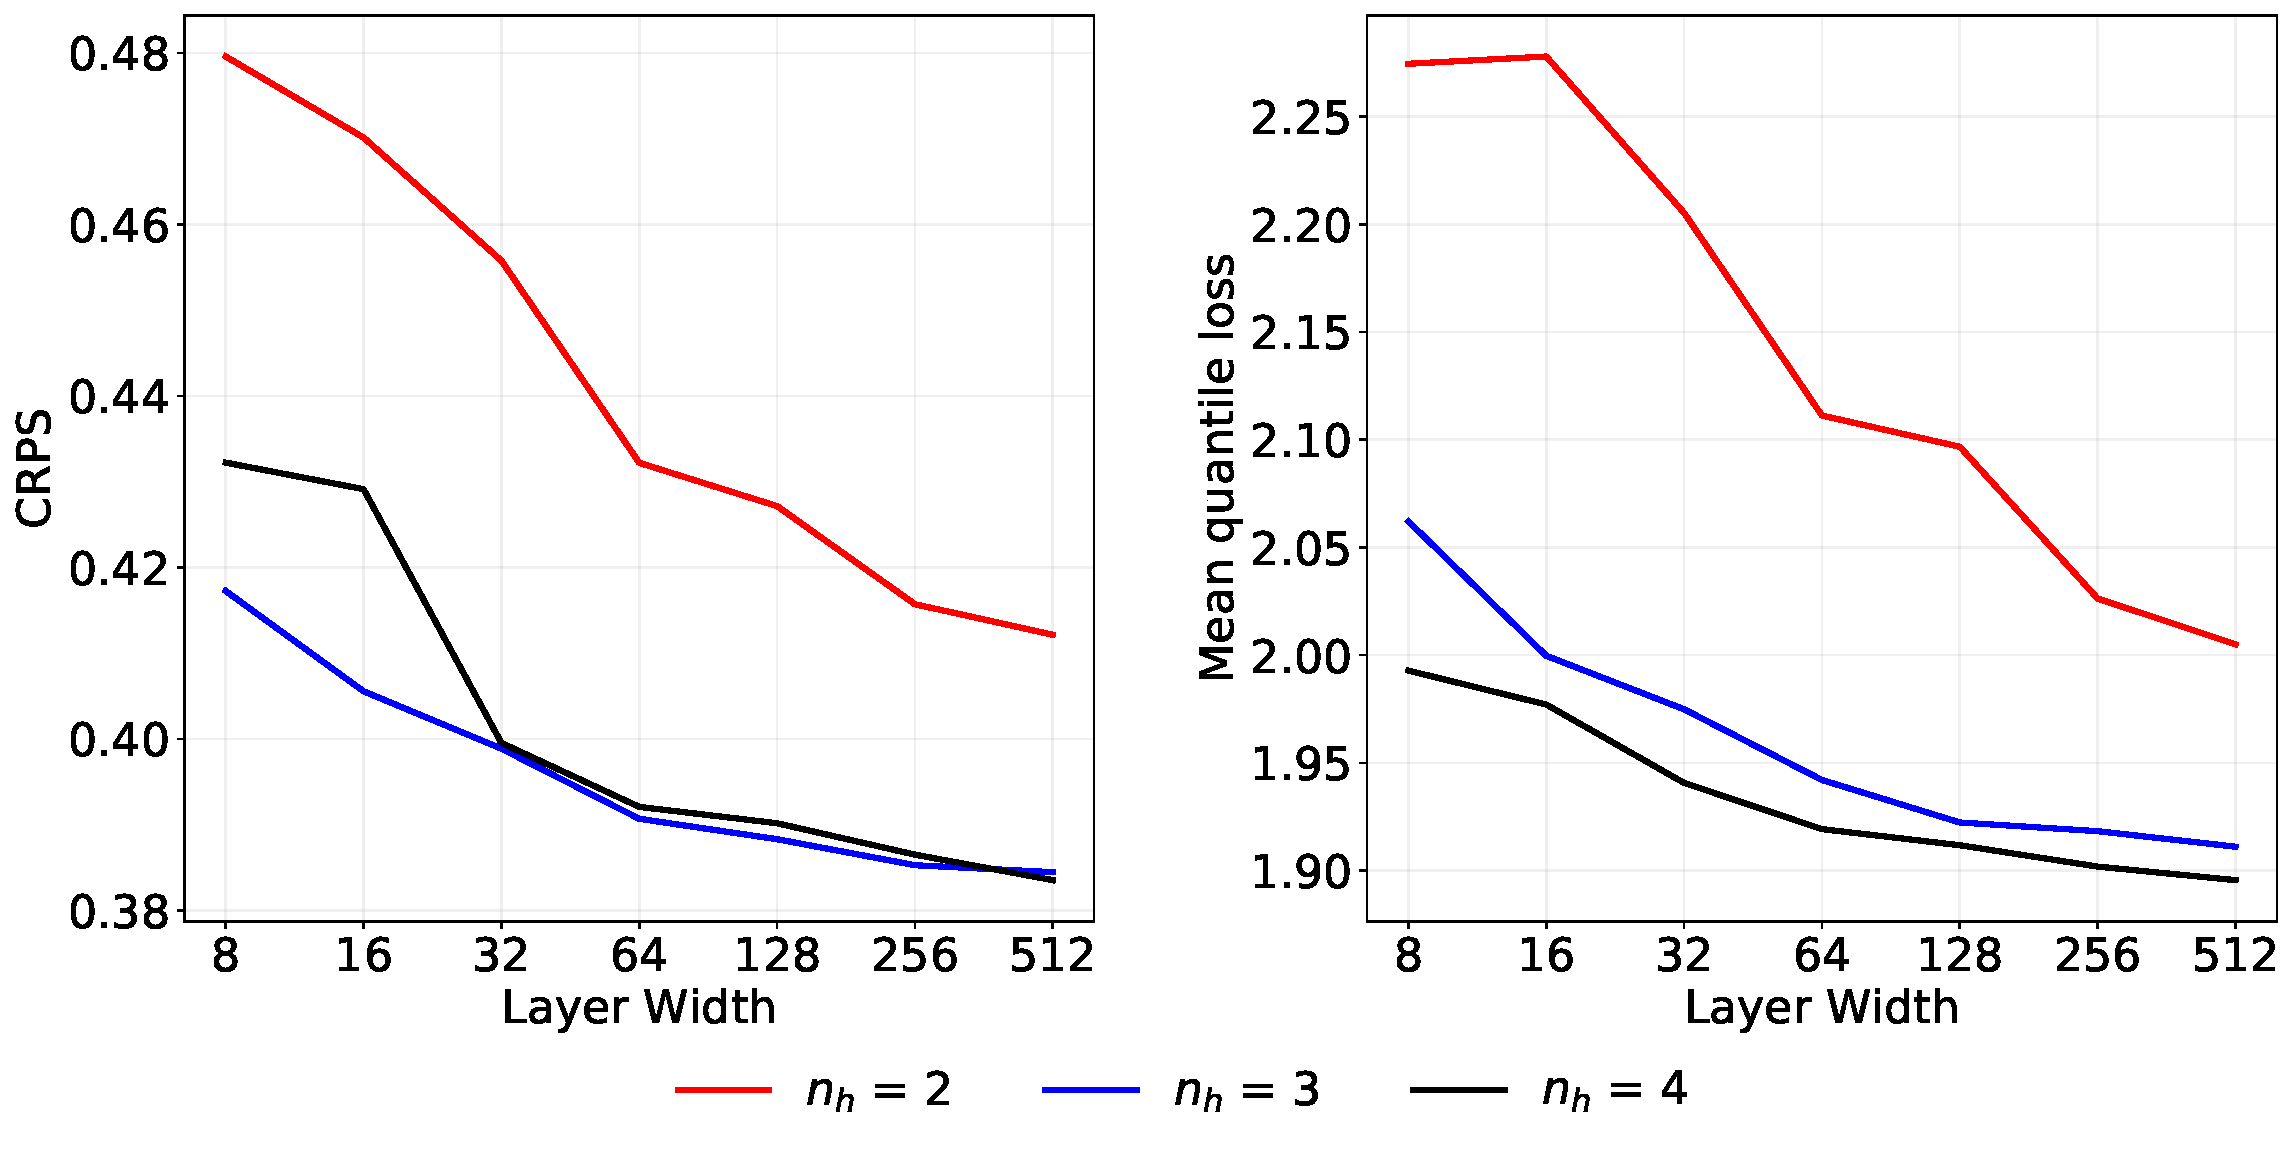
\includegraphics[height=60mm]{Figures/CRPS.pdf} 
	\caption{CRPS(left) and mean quantile loss(right) averaged over all predicted quantiles for different combinations of layer width and hidden layers ($n_h$). The results are from QRNN-single applied to I2V.}
	\label{fig:grid_search}	
\end{figure*}
In this study, we investigated the performance of QRNN only to certain hyper-parameters like number of neurons, hidden layers, learning rate, convergence epochs and batch size. The optimization of other hyper-parameters was not performed and were chosen empirically. Firstly, we performed a grid search to define the structure of the neural network. We evaluated the performance for three sizes of hiddden layers($n_h$ = 2, 3, 4), and layer widths of sizes in the set [8, 16, 32, 64, 128, 256, 512]. The mean quantile loss and CRPS over all predicted quantiles was computed for each configuration (Fig.~\ref{fig:grid_search}). Increasing the complexity of the network by increasing the layer width and depth has a positive impact on performance. However for four hidden layers, increasing the number of neurons beyond 128 has no significant impact on the performance. On basis of these results, a neural network with four hidden layers and 128 neurons in each layer is selected. For optimising the training parameters, a customised  learning rate scheduler was implemented. The initial learning rate was reset after a certain number of epochs.  We started the training process with a initial learning rate of 0.1, and decreased it by a factor of 10 after 100 epochs. The best neural network performance was obtained when the network was trained three times. Each time with a new initial learning rate. For each training, if the validation loss remained unchanged till 6 training epochs, the learning rate was reduced by a factor of 2. 
In order to select the batch size, we simply compared the performance for two batch sizes: 128 and 256, and the former gave better results. Concerning number of epochs, we obtained best results when the network was trained longer. Choosing a lower value of epochs (e.g. 50), did not affect the accuracy of the median value, yet deteriorated the prediction uncertainty. We did not optimise the type of activation function and Rectified Linear Unit (ReLu) was used in all layers. 

Though these set of hyper-parameters were selected for QRNN-single applied to I2V, they worked well for other QRNN models and their multiple configurations. All the results described in this study use an identical hyper-parameter configuration.


\subsection{ICI}
\subsubsection{Example results}
%
%f
\begin{figure}[t]
	\centering
	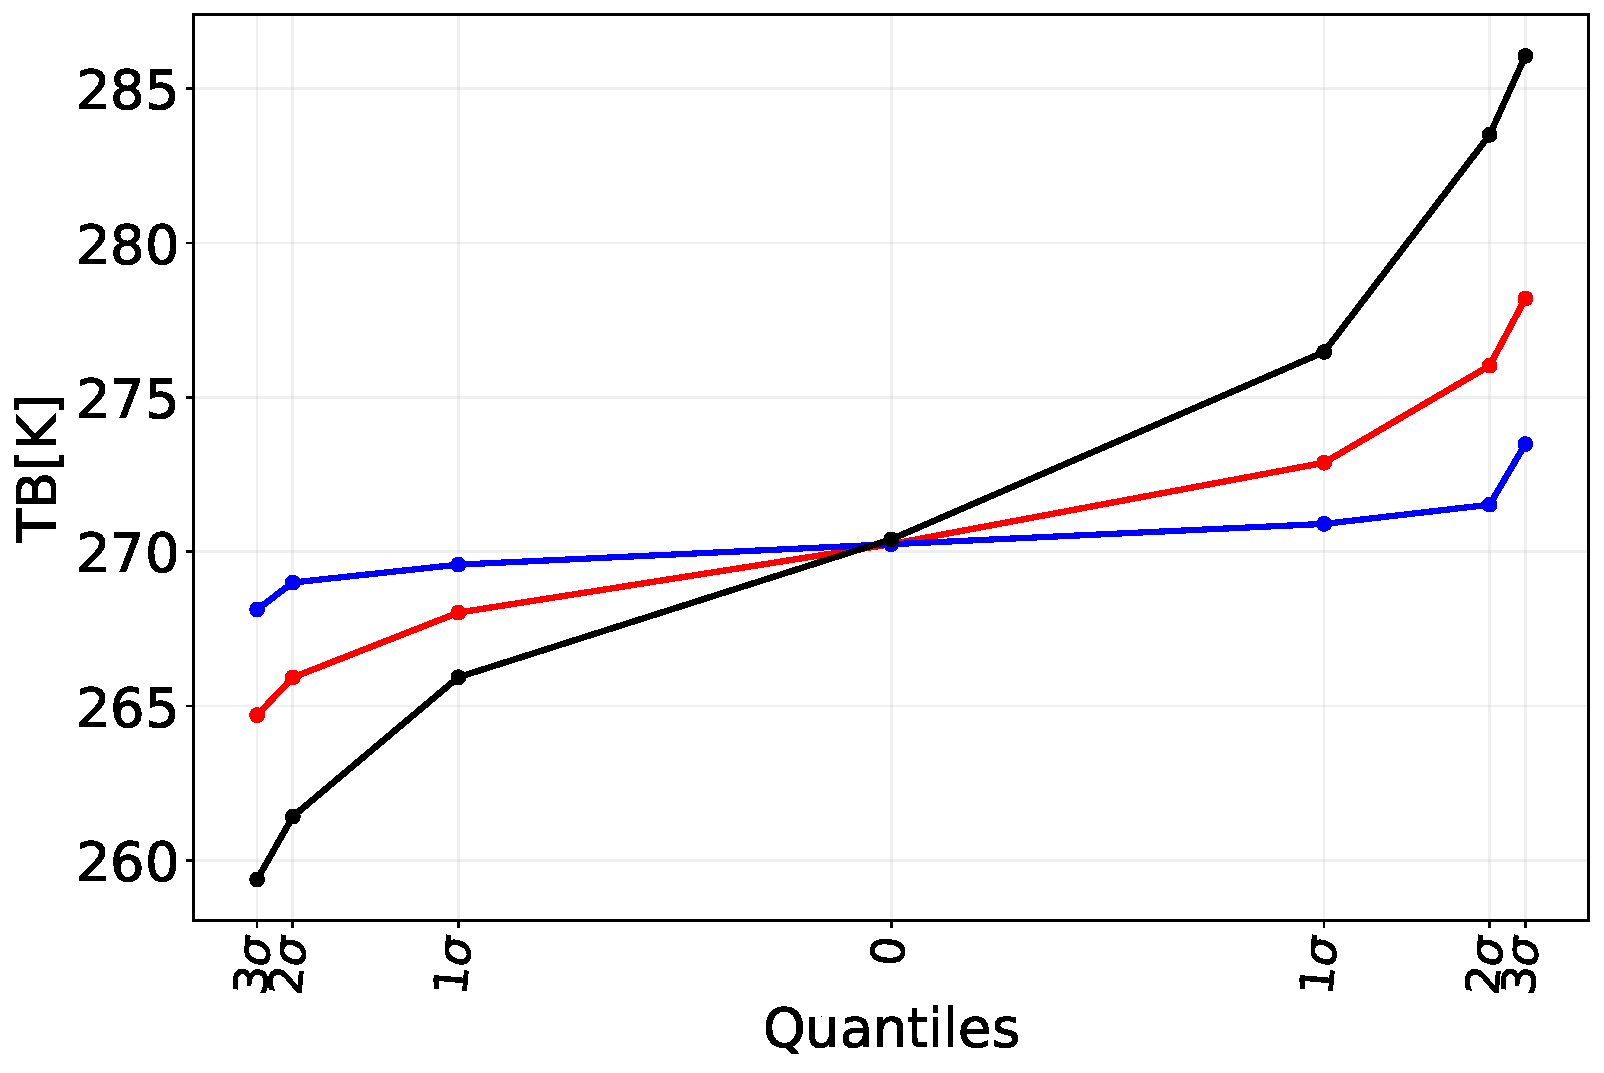
\includegraphics[height=60mm]{Figures/posterior_distribution_I1V.pdf} 
	\caption{Predicted quantiles of the conditional distribution of $\ynfcs$ for
		the ICI I1V channel.}
	\label{fig:posterior_distribution_I1V}	
\end{figure}
%f
\begin{figure*}[t]
	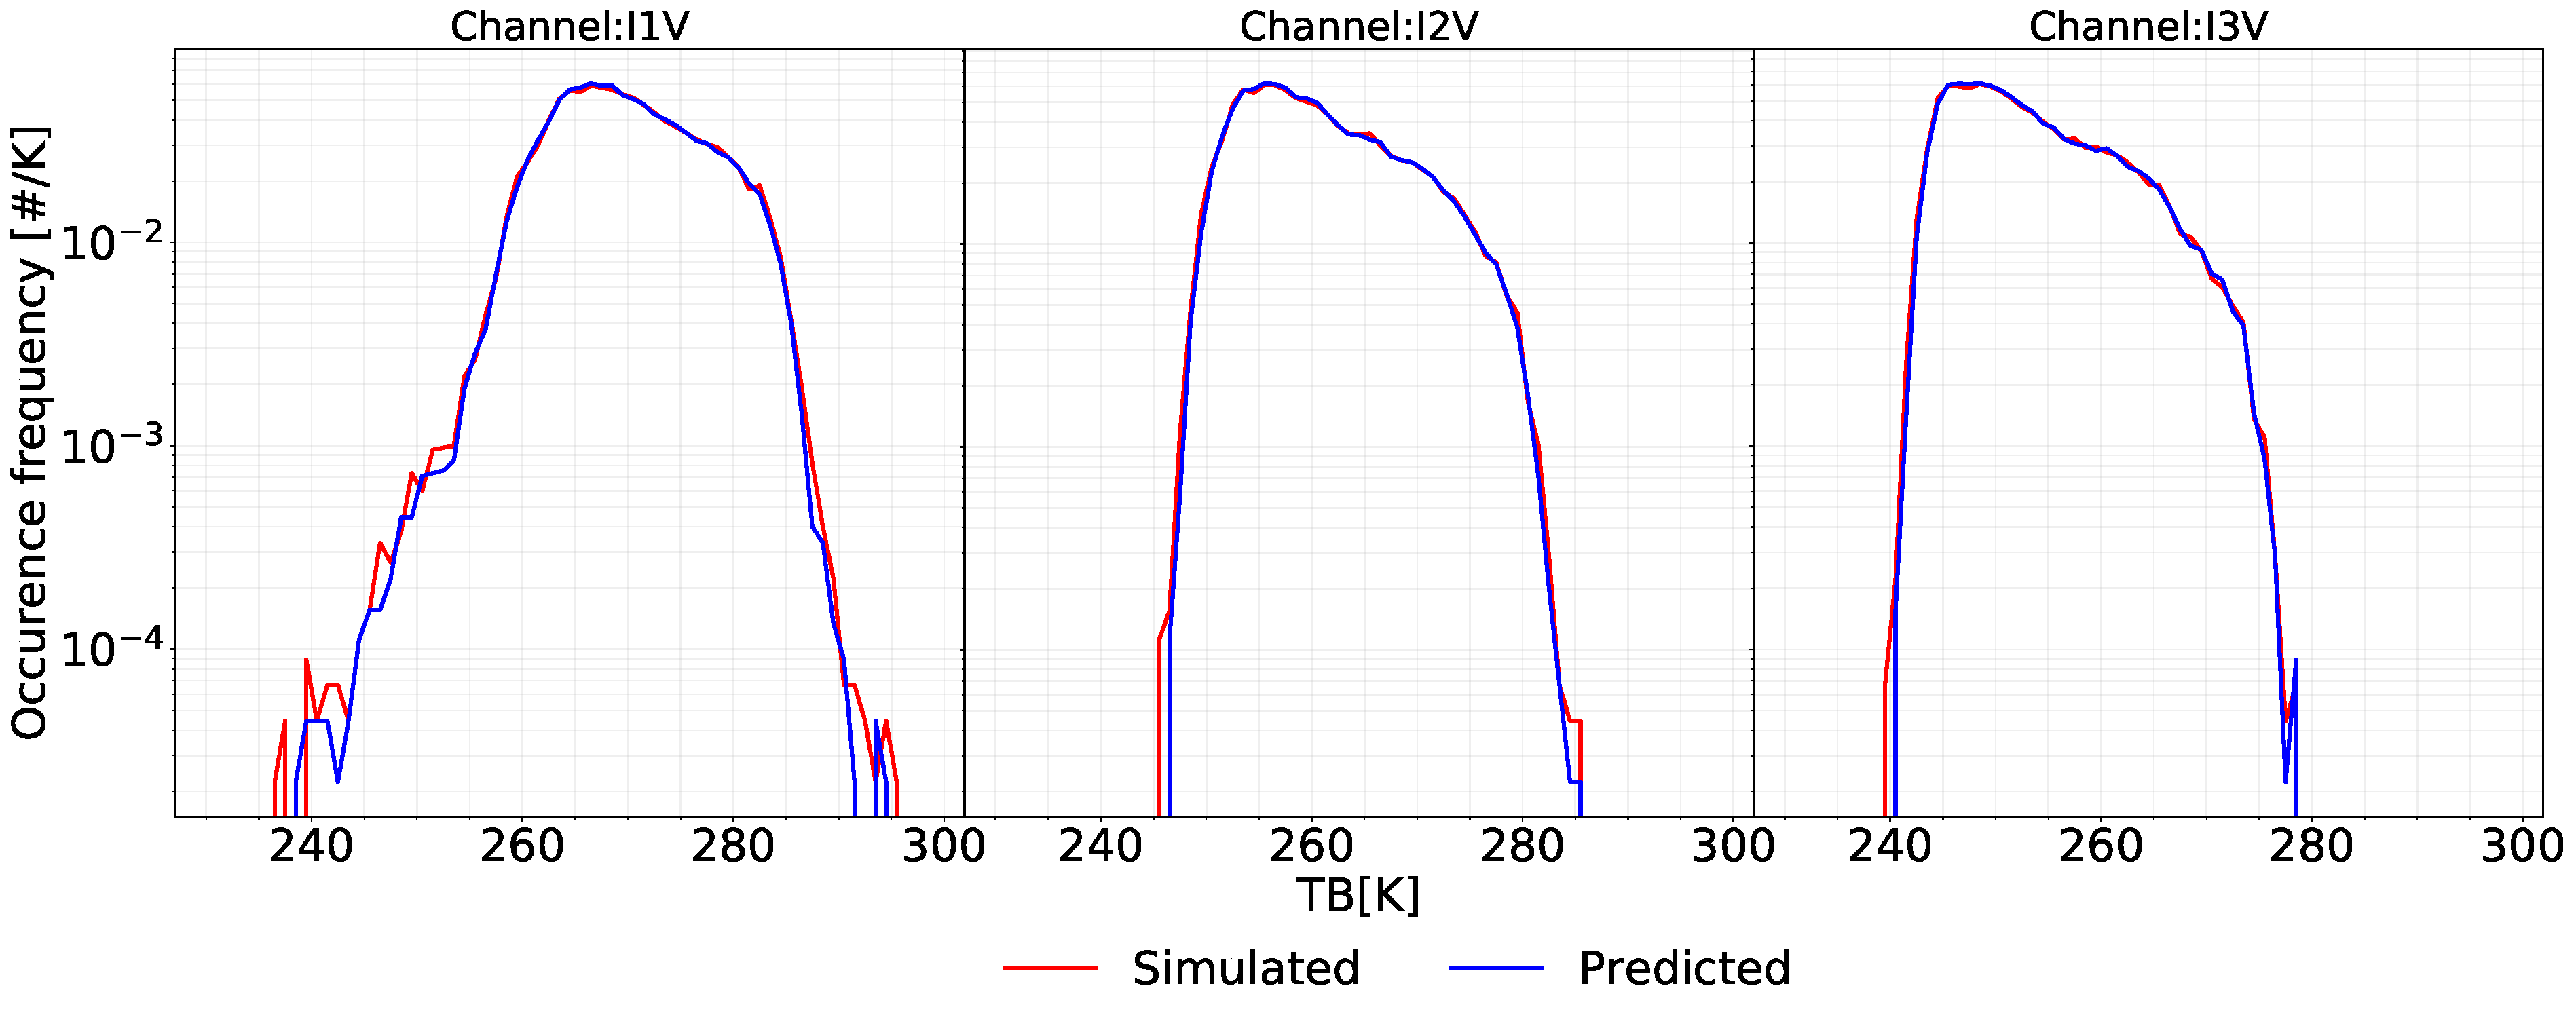
\includegraphics[width=\textwidth]{Figures/PDF_predictions_ICI.pdf} 
	\caption{Distributions of point estimate NFCS from QRNN-single for channels I1V, I2V and I3V. The corresponding distributions for NFCS simulations are also shown.}
	\label{fig:PDF_predictions}	
\end{figure*}

Fig.~\ref{fig:posterior_distribution_I1V} presents examples of the predicted quantiles for three different corrected observations of the ICI I1V channel. The three cases have a similar median value but very different spread of the remaining quantiles. These examples illustrate the case of very similar corrected observation values (the estimated median) but with different estimated observation errors.
For an analysis of QRNN predictions, a point estimate of the posterior distribution is required. Usually for Bayesian analysis, the posterior mean or posterior median are selected as point estimates. In this study, we assume the posterior median to be the best estimate for the predicted NFCS value. The distribution of point estimates is shown in Fig.~\ref{fig:PDF_predictions}. For all three channels, an excellent agreement between the predictions and simulations is observed. This indicates that QRNN is successful in predicting NFCS values for majority of the cases. At lower brightness temperatures, the frequency of predictions is slightly smaller than simulations. This could be due to few QRNN predictions ending up with partially corrected cloud impact. 
 
\subsubsection{Analysis of cloud filtering}
%
\label{sec:cloud_filtering}
%f 
\begin{figure*}[t ]
	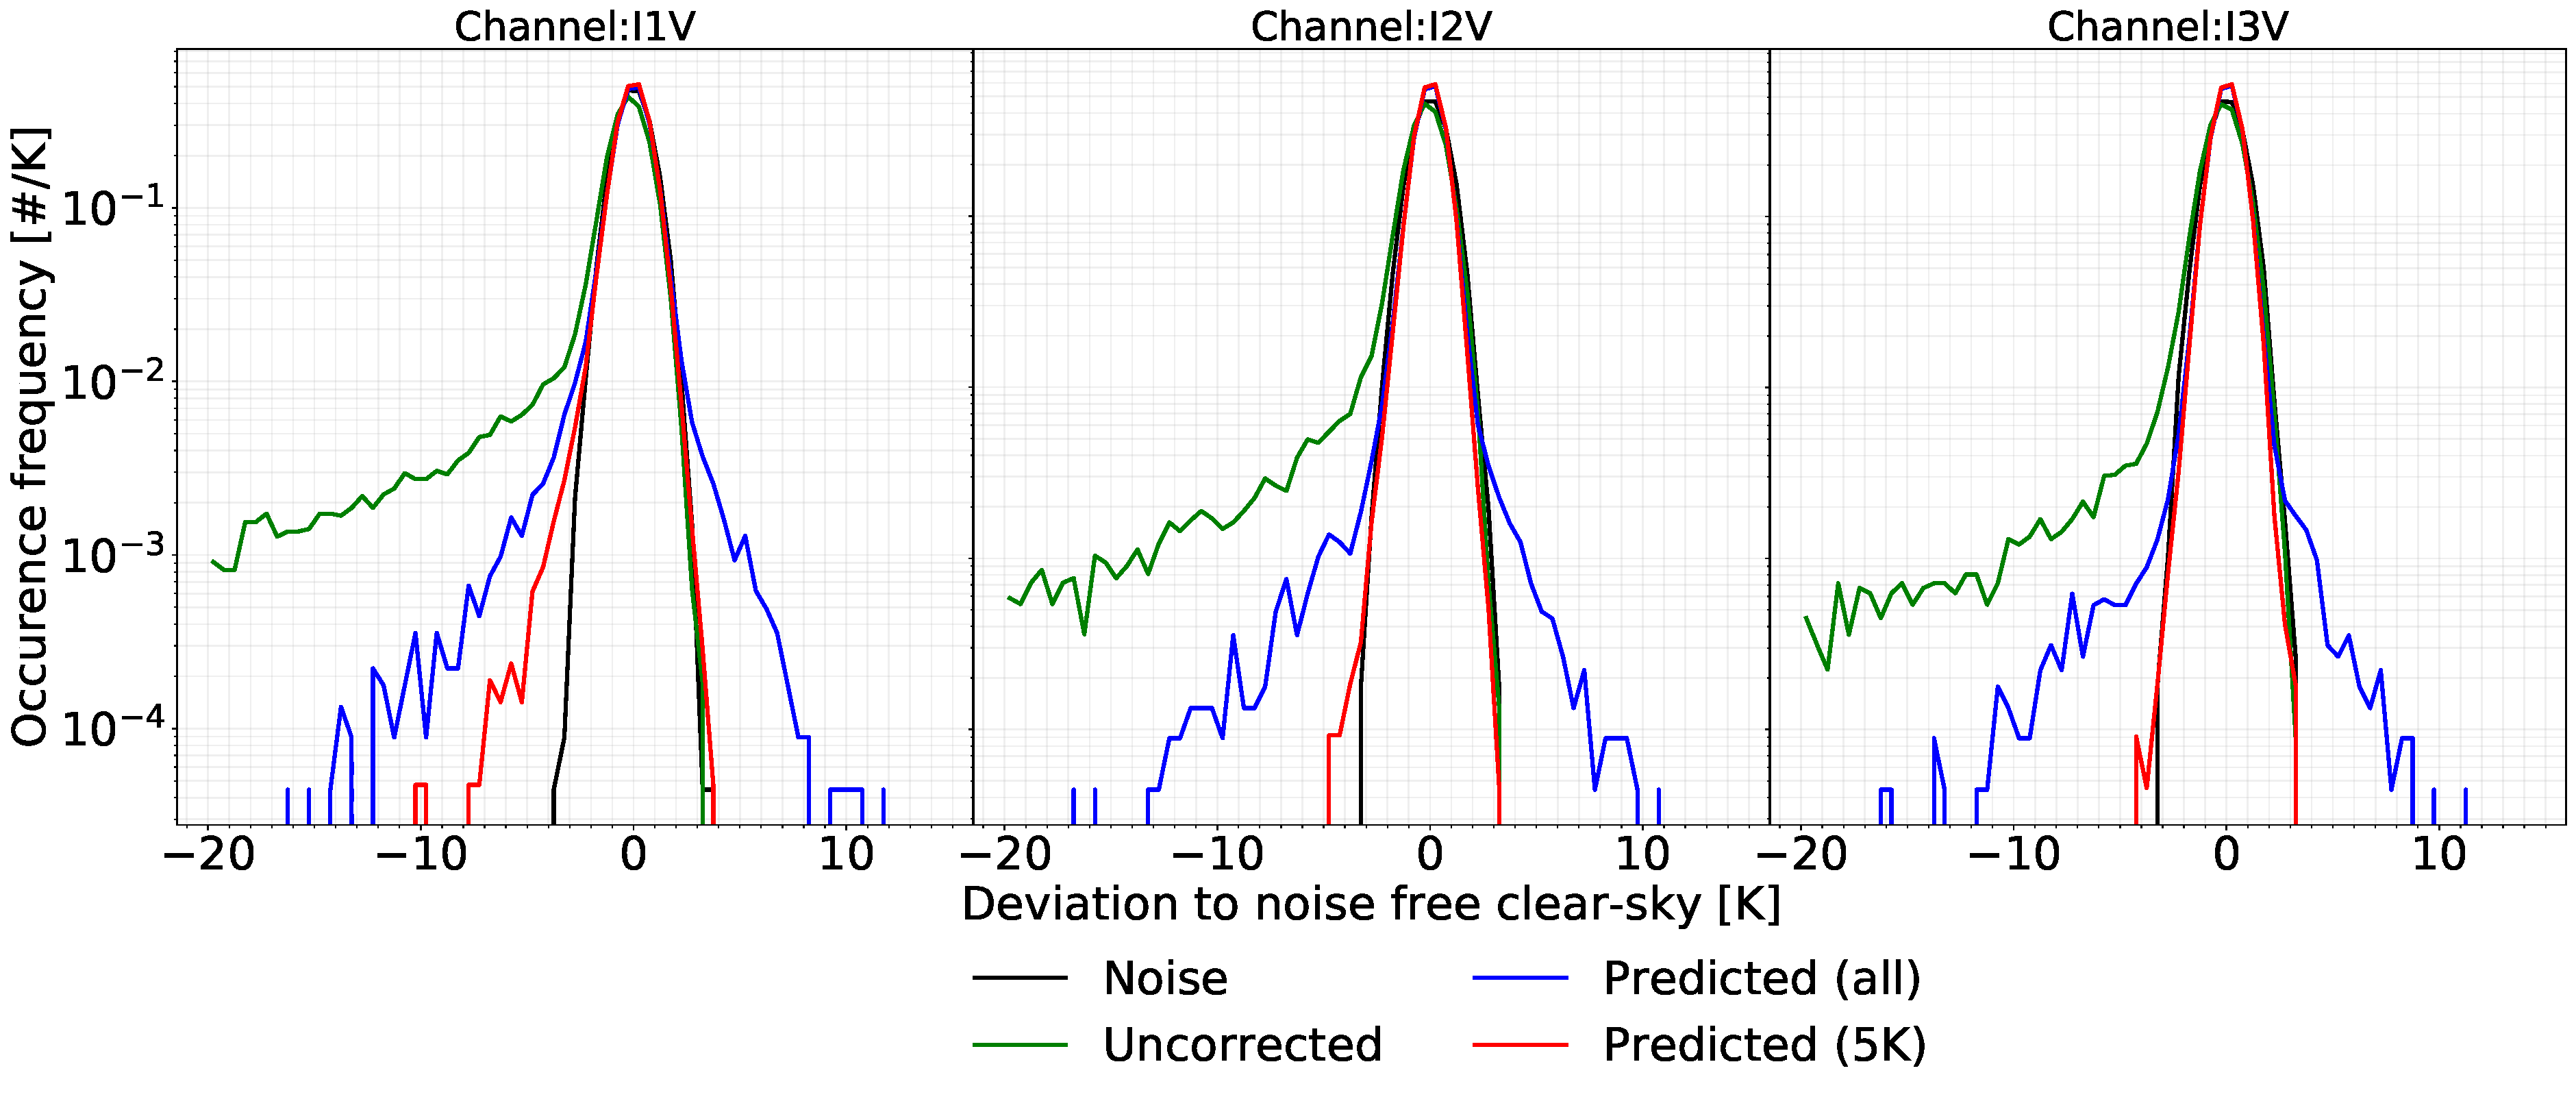
\includegraphics[width=\textwidth]{Figures/error_distribution_QRNN-single.pdf} 
	\caption{Error distributions for deviations of filtered and predicted data to NFCS simulations. The results are from QRNN-single and channels I1V, I2V and I3V. Noise for each channel is also plotted for reference. The label ``Uncorrected'' represents the measurement data and ``Filtered(5\,K)'' represents the dataset when no correction is made but cases with cloud correction greater than 5\,K are rejected. ``Predicted(All)'' denotes the entire prediction dataset, while ``Predicted(5\,K)'' refers to the predicted dataset but where cases with cloud correction greater than 5\,K are excluded.}
	\label{fig:error_distributions}	
\end{figure*}
\begin{table*}[t]
	\caption{ Error statistics for deviations of filtered and predicted data to NFCS simulations. 
		The values for Bias, mean absolute error(MAE), standard deviation(STD), and measure of skewness(Skewness) are shown. Results are from both QRNN-single and QRNN-all and for channels I1V, I2V and I3V. The number in parentheses is the percentage of cases removed by filtering. The label ``Filtered(5\,K)'' represents the dataset when no correction is made but cases with cloud correction greater than 5\,K are rejected, ``Predicted(All)'' refers to the complete predicted dataset, while ``Predicted (5\,K)'' denotes the prediction dataset but where cases with cloud correction greater than 5\,K are excluded.}
	\label{tab:error_statistics_ici}
	%	\tabcolsep=0.11cm
	\begin{tabular}{llrr|rrr|rrr}
		\tophline
		&&\multicolumn{2}{c|}{Simulations}& \multicolumn{3}{c|}{QRNN-single} & \multicolumn{3}{c}{QRNN-all}\\
		\cline{3-10}
		%		\hline
		&&   Clear-sky &   All-sky &  Filtered & Predicted & Predicted &   Filtered & Predicted & Predicted \\
		&&&&							(5\,K) &(All)& (5\,K) & (5\,K)&(All)& (5\,K)\\
		\middlehline
		%		\multicolumn{7}{c}{Channel - I1V}\\
		
		I1V& Bias     &  0.00 & -1.88 & -0.32(6.1\%) & -0.06 & -0.04 & -0.31(6.1\%) & -0.06 & -0.04 \\
		&MAE      &  0.64 &  2.32 &  0.79 &  0.64 &  0.55 &  0.78 &  0.61 &  0.54 \\
		&STD      &  0.80 &  8.84 &  1.07 &  0.98 &  0.73 &  1.07 &  0.91 &  0.71 \\
		&Skewness & -0.01 & -8.10 & -1.53 & -1.53 & -0.75 & -1.52 & -1.07 & -0.55 \\
		\middlehline
		I2V &Bias     & -0.00 &  -1.04 & -0.24(3.7\%) & -0.01 & -0.00 & -0.24(3.6\%) & -0.05 & -0.03 \\
		&MAE      &  0.64 &   1.52 &  0.74 &  0.52 &  0.46 &  0.75 &  0.44 &  0.39 \\
		&STD      &  0.80 &   5.95 &  0.99 &  0.82 &  0.59 &  0.99 &  0.67 &  0.50 \\
		&Skewness &  0.00 & -10.80 & -1.10 & -2.17 & -0.27 & -1.05 & -2.22 & -0.27 \\
		\middlehline	
		I3V &Bias     & -0.00 &  -0.63 & -0.18(2.3\%) &  0.01 &  0.02 & -0.19(2.2\%) & -0.03 & -0.03 \\
		&MAE      &  0.64 &   1.15 &  0.71 &  0.51 &  0.47 &  0.72 &  0.46 &  0.42 \\
		&STD      &  0.80 &   4.27 &  0.93 &  0.77 &  0.59 &  0.95 &  0.68 &  0.54 \\
		&skewness & -0.00 & -13.41 & -0.86 & -1.75 & -0.11 & -0.93 & -1.53 & -0.14 \\
		\bottomhline
	\end{tabular}
	\belowtable{} % Table Footnotes
\end{table*}

In this section, we use the point estimates to formulate a cloud filtering scheme. All cases with  cloud correction greater than a certain threshold are classified as cloudy and omitted from the dataset. Cloud correction is calculated as the difference of the point estimate to the corresponding measurement. Since this is a pure-filter, for the cases classified as clear-sky, the a priori values are used instead of the point estimates. 

To implement the cloud filtering scheme, we chose 5\,K cloud correction as the filtering threshold. All cases with correction greater than 5\,K were rejected. In order to analyse the performance of the filtering threshold, the deviations of the filtered measurements to the NFCS simulations were calculated. Fig.~\ref{fig:error_distributions} shows the distribution of the deviations for filtered(red) and original datasets(green). Cloud contamination causes a reduction in the brightness temperatures, and introduces a large negative bias in the error distributions. Without any cloud impact, the error distributions must follow a Gaussian distribution with a narrow spread. When filtering is activated, the resulting distributions have a low but asymmetric spread. The right side of the distributions follows the measurement noise, as expected, but the left side has a significantly smaller negative skewness than the measurements. This indicates that 5\,K filter can successfully remove cases associated with high cloud impact. However at the same time, the asymmetric error distribution is a result of cases erroneously classified as clear-sky. 

For a quantitative assessment of the performance achieved with cloud filtering, we calculated the average error bias, MAE (mean absolute error) and standard deviation of the deviations. The asymmetry of error distributions around their mean is also calculated through the measure of skewness. Fisher-Pearson coefficient of skewness is used to calculate the measure of skewness: 
\begin{equation}
g_1 = \frac{m_3}{m_2^{3/2}}, 
\end{equation}
where $m_2$ and $m_3$ are biased sample's second and third central moments. The error metrics corresponding to the error distributions described in Fig.~\ref{fig:error_distributions} are provided in Table~\ref{tab:error_statistics_ici} under label "Filtered(5\,K)". The average bias in I1V measurements is -1.88\,K, and rejecting around 6\% of the cases as cloudy, reduces the bias to -0.32\,K. The standard deviation also reduces to 1.07\,K from 8.84\,K. Similarly for I2V, the average error bias in all sky measurements is -1.04\,K, that reduces to -0.24\,K after filtering. The corresponding improvement in MAE is almost 65\%. Only 3.7\% of the total cases are rejected to achieve this accuracy. For I3V, filtering classifies 2.3\% of the total cases as cloudy and reduces the bias to 0.18\,K from -0.63\,K and the standard deviation from 5.95\,K to 0.91\,K. The results from QRNN-all are also shown in the same table. Using all 183\,GHz channels concurrently has no notable impact on the cloud filtering. Almost similar statistics are obtained from both models.

Overall for all three channels, the notable decrease in the errors indicates that the cloud filter is effective in removing most of the cloudy cases, however few cases with low cloud impact still pass through the filter and deteriorate the performance. Thus pure-filtering approach can prove as a reliable procedure for removing cases with high cloud impact, but additional measures are needed to remove cases with low cloud impact.

A lower filtering threshold can help alleviate this problem to certain extent, however that can come at the cost of high rejection rate. We investigated the performance of cloud filtering with different threshold values. Fig.~\ref{fig:filtering_thresholds} shows the average errors obtained from different filtering thresholds and the corresponding percentage of data omitted. Lowering the filtering threshold from 5\,K to 2.5\,K has only a small effect on the filter performance. However, a further decrease in the filtering threshold decreases the average error bias significantly, albeit with a high rejection rate. For example for I1V, when all cases with cloud correction greater 0.5\,K are filtered, the mean error bias of the subset is -0.06\,K, MAE is 0.59\,K and the standard deviation is 0.75\,K. Though, these values are comparable to the NFCS simulations, the high performance comes at the cost of rejecting more than 30\% of the total cases. The high fraction of rejection is a consequence of clear-sky cases being erroneously classified as cloudy. Since QRNN gives out NFCS values, choosing an unusually low correction threshold can also classify noisy clear-sky cases as cloudy. 

\begin{figure}[t]
	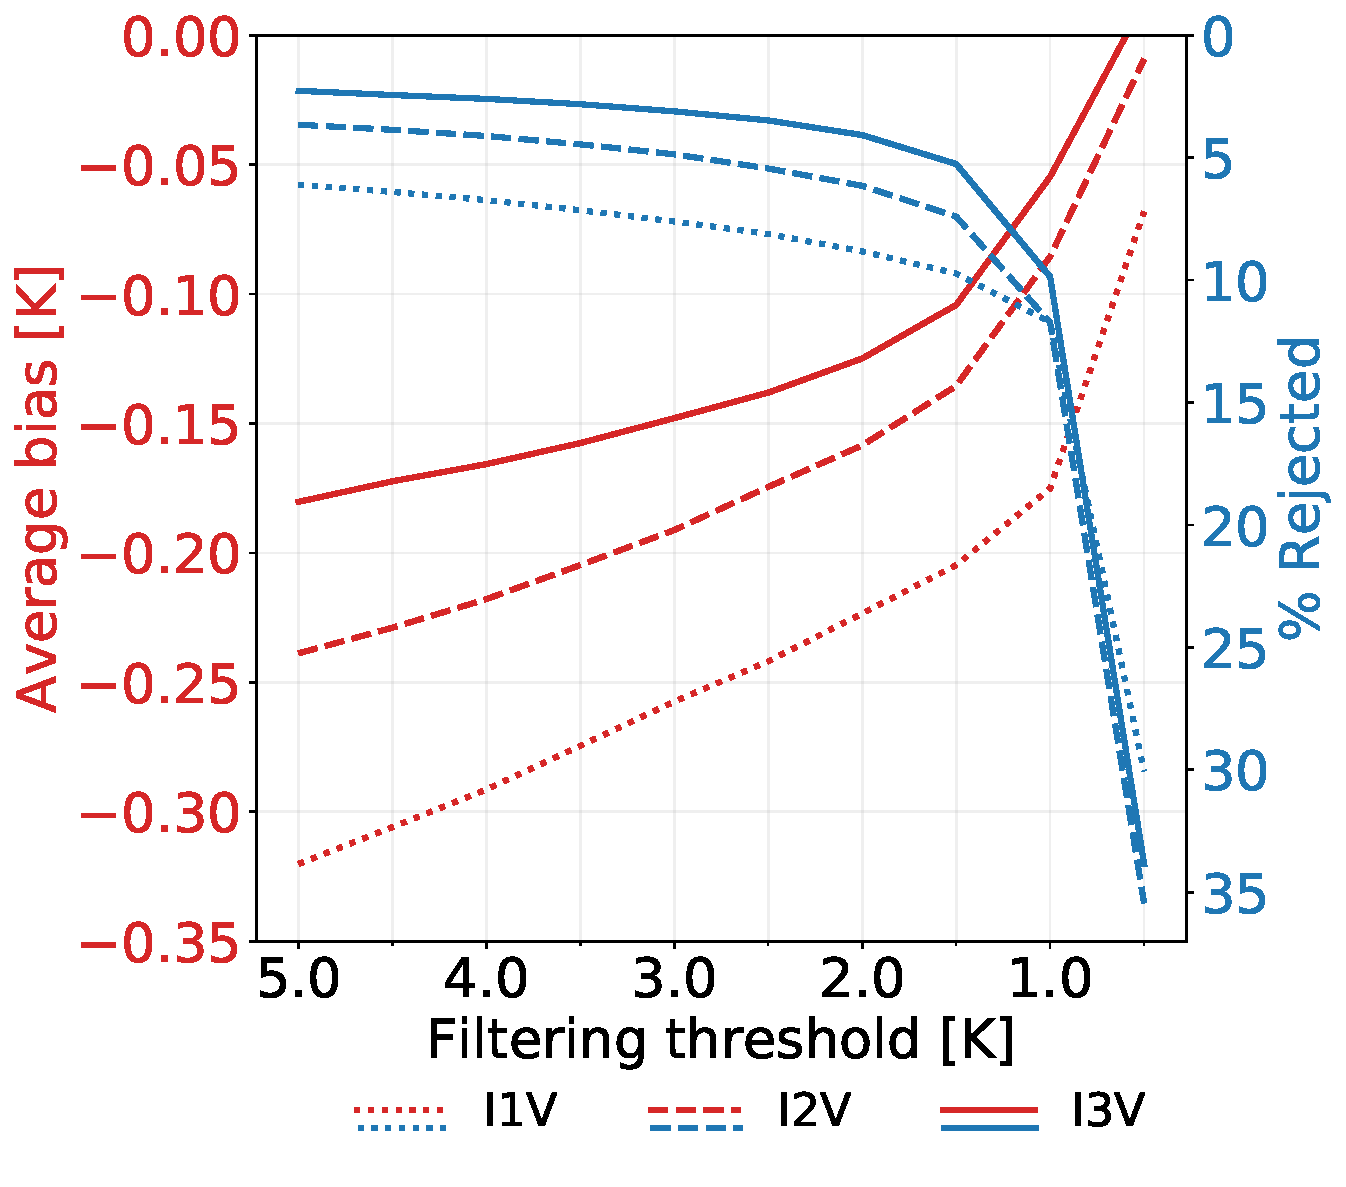
\includegraphics[width=70mm]{Figures/different_filtering_thresholds.pdf} 
	\caption{A comparison of the  average bias when pure-filtering approach is applied with different thresholds (red curves). The corresponding fraction of cases rejected is also shown on the right y-axis(blue curves). The results are from QRNN-single. }
	\label{fig:filtering_thresholds}	
\end{figure} 

\subsubsection{Error of best estimate}  
%
%t
\begin{table*}[t]
	\caption{A comparison of the error statistics from QRNN-single and QRNN-all, when only cases with cloud correction greater than 10\,K are included. The number in the parentheses gives the fraction of cases included.}
	\label{tab:error_statistics_ici_high_cloud_impact}
	%	\tabcolsep=0.11cm
	\begin{tabular}{lrr|rr|rr}
		\tophline
		&\multicolumn{2}{c|}{I1V}& \multicolumn{2}{c|}{I2V} & \multicolumn{2}{c}{I3V}\\
		\cline{2-7}
		&QRNN-single& QRNN-all & QRNN-single & QRNN-all  & QRNN-single & QRNN-all\\
		\middlehline
		Bias     & -0.53(4.02\%) & -0.38(4.07\%)  & -0.42(2.26\%) & -0.46(2.25\%) & -0.25(1.32\%) & -0.40(1.28\%) \\
		MAE      &  2.32 &  1.93  &  2.77 &  2.08 &  3.10 &  2.59 \\
		STD      &  3.13 &  2.63  &  3.65 &  2.85 &  4.03 &  3.47 \\
		\bottomhline
	\end{tabular}
	\belowtable{} % Table Footnotes
\end{table*}

The QRNN prediction accuracy is estimated by computing the deviation of the best estimate to its corresponding NFCS simulation(Fig.~\ref{fig:error_distributions}). The predicted values have symmetric error distributions albeit with a large spread. The large spread on the left is due to cases which end up with incomplete cloud correction, while the spread on the right is from cases where the predicted values are warmer than the simulations. For all three channels, quite similar behaviour is observed, though I1V has the most cases with residual cloud impact. If the predicted cases with correction more than 5\,K are rejected, the resulting error distributions fit the measurement noise, except for I1V, where cases with residual cloud impact introduces a negative bias. 

For a quantitative assessment of the errors, we calculated the error metrics described in Sect.~\ref{sec:cloud_filtering} and the results are displayed in Table~\ref{tab:error_statistics_ici}. The average bias in I1V measurements is -1.88\,K, which reduces to -0.06\,K after cloud correction. The corresponding standard deviation is 0.98\,K in comparison to 8.84\,K in the measurements. The prediction accuracy of QRNN-single is further higher when filtering is made on the predictions. In this case, the residual bias is only -0.04\,K, and the standard deviation is 0.73\,K, which is in fact of the order of measurement noise (0.80\,K). Similar results are seen for I2V, though a better performance is observed. In I2V, the measurement bias is -1.04\,K which reduces to -0.01\,K after correction. The MAE reduces from 1.52\,K to 0.52\,K. Removing cases with correction greater than 5\,K from the predictions removes 3.7\% of the data and reduces the absolute error to 0.46\,K. The standard deviation of the resulting dataset is only 0.59\,K as compared to 0.80\,K from noise. The reduction in the variability is also evident in the Fig~\ref{fig:error_distributions}, where the peak of distributions is sharper. In comparison to I1V and I2V, I3V has the lowest fraction of the measurements with significant cloud impact. In the predicted dataset, the bias is 0.01\,K and the MAE is 0.51\,K. Including correction along with filtering reduces the MAE further down to 0.47\,K and standard deviation to 0.59\,K, which is again smaller than that of noise(0.80\,K).  

Next, we describe the results from QRNN-all. In this model, all 183\,GHz channels along with other sub-mm channels are included while training. This model is designed to identify if other channels of the same frequency can provide auxiliary information in the training process. The results from QRNN-all all are provided in the last columns of Table~\ref{tab:error_statistics_ici}. For I1V, using additional information from other two 183\,GHz channels has only a slight positive impact on the predictions. In the prediction dataset, the average bias for QRNN-all and QRNN-single is identical, but the MAE in QRNN-all are almost 4.5\% less than QRNN-single. However when the predictions are filtered with 5\,K threshold, the performance of both models is quite similar. This indicates that information from other channels is only slightly helpful in improving the correctness of cases associated with high cloud impact. The predictions for cases with low cloud impact have no significant gain. For I2V, the predictions from QRNN-all have a slightly worse average error bias than QRNN-single, yet a significant improvement in the prediction accuracy is observed. When all predictions are considered, the MAE is 0.44\,K in comparison to 0.52\,K from QRNN-single, showing an improvement of almost 15\%. Similarly the standard deviation of the errors is only 0.67\,K, which is notably smaller than the measurement noise. Additionally, when the predicted dataset is filtered with 5\,K threshold, the accuracy is even better. The MAE reduces to 0.39\,K and standard deviation to 0.50\,K. This implies that cases pertaining to clear-sky conditions and relatively low/no cloud impact benefit the most from the auxiliary information. This is in contrast to I1V, where accuracy of such cases remained unaffected. For I3V, the performance of QRNN-all is comparable to that for I2V. For I3V, the MAE in QRNN-all is 0.46\,K compared to 0.51\,K from QRNN-single, and the corresponding standard deviations are 0.68\,K and 0.77\,K. Removing the cases with cloud impact greater than 5\,K from the predictions, leads to no change in the average bias, but the MAE and standard deviation reduce by almost  8\% and 20\% respectively. This is again a consequence of improved prediction accuracy of cases with low/no cloud impact.  

In order to quantify the positive effect of QRNN-all on cases with high cloud impact, the error statistics for all cases with cloud correction greater than 10\,K were computed (Table~\ref{tab:error_statistics_ici_high_cloud_impact}). For I1V, only 4\% of the cases have cloud correction greater than 10\,K, but very low prediction accuracy. QRNN-all improves the overall error bias from -0.53\,K to -0.38\,K and the standard deviation from 3.13\% to 2.63\%, but is unsuccessful in removing the cloud impact completely. A likewise improvement is also observed for I2V. Despite both models being only partially successful in removing the cloud impact, QRNN-all has a better performance among the two. For I2V, such cases form only 2.25\% of the testing dataset. Predictions from QRNN-all have slightly worse values for average error bias, but both MAE and standard deviation improve by over 20\%. For I3V also, the cases with high cloud impact, though very low in number, also gain positively from the auxiliary information. 


The results show that both QRNN-single and QRNN-all are successful in predicting NFCS values for I2V, and I3V, and partially successful for I1V. The resulting error distributions are symmetric with low bias and standard deviation. For I2V and I3V, the variability of errors is even smaller than the noise. This is a consequence of predictions for cases associated with clear sky conditions. QRNN predictions are weighted mean of measurements between channels. For clear-sky conditions, the averaging of cases observed by multiple channels can cancel out the noise. The cancelling of noise is stronger in QRNN-all as all 183\,GHz channels are used concurrently. The lower prediction accuracy of I1V can be explained by the fact that it is the outermost 183\,GHz channel. The other sub-mm channels cannot provide a full coverage for the hydrometeor impact in I1V. Depending upon the atmospheric scenarios, there is always a portion of data detected by I1V, but never seen by any other channel. Though such cases are few, QRNN cannot learn to predict the clear-sky values accurately for cases which lie outside the coverage area. Besides this, lower representation of high cloud impact cases in the training set also affects QRNN accuracy.
 

\subsubsection{Uncertainty quantification}
\label{sec:prediction_uncertainty}
%f 
\begin{figure}[t]
	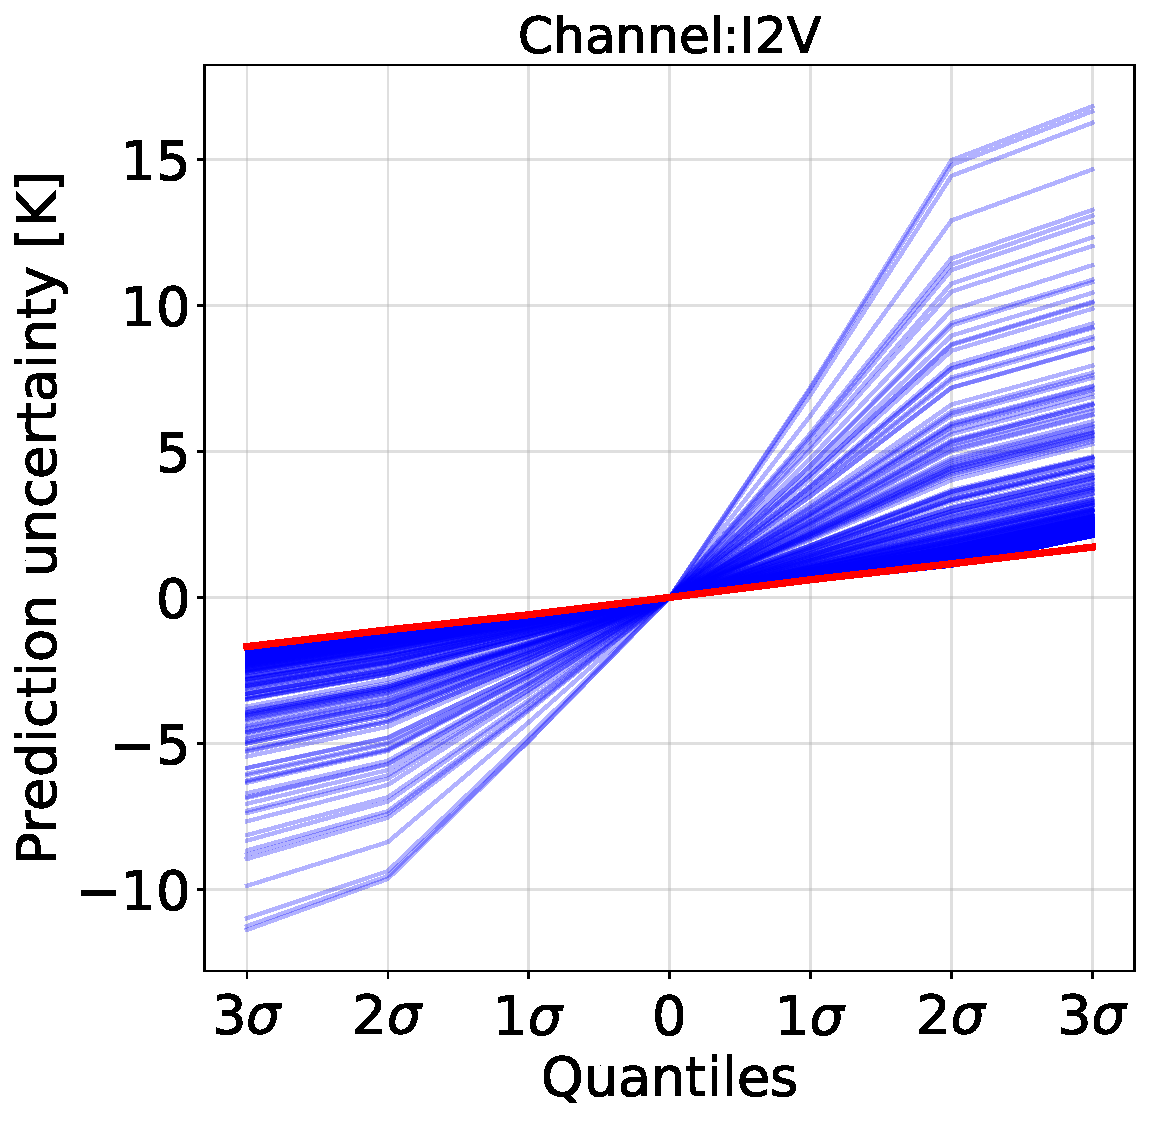
\includegraphics[width = 70mm]{Figures/prediction_uncertainty_I2V.pdf}	
	\caption{The prediction uncertainty  for QRNN-single(I2V) with respect to quantiles for randomly selected 1500 cases. The quantiles have been plotted at equidistant points. The black line represents a hypothetical Gaussian distribution of $270\pm0.60$\,K, which is of the order of standard deviation for I2V predictions (see Table~\ref{tab:error_statistics_ici}).}
	\label{fig:prediction_uncertainty_I2V}	
\end{figure}
\begin{figure*}[t]
	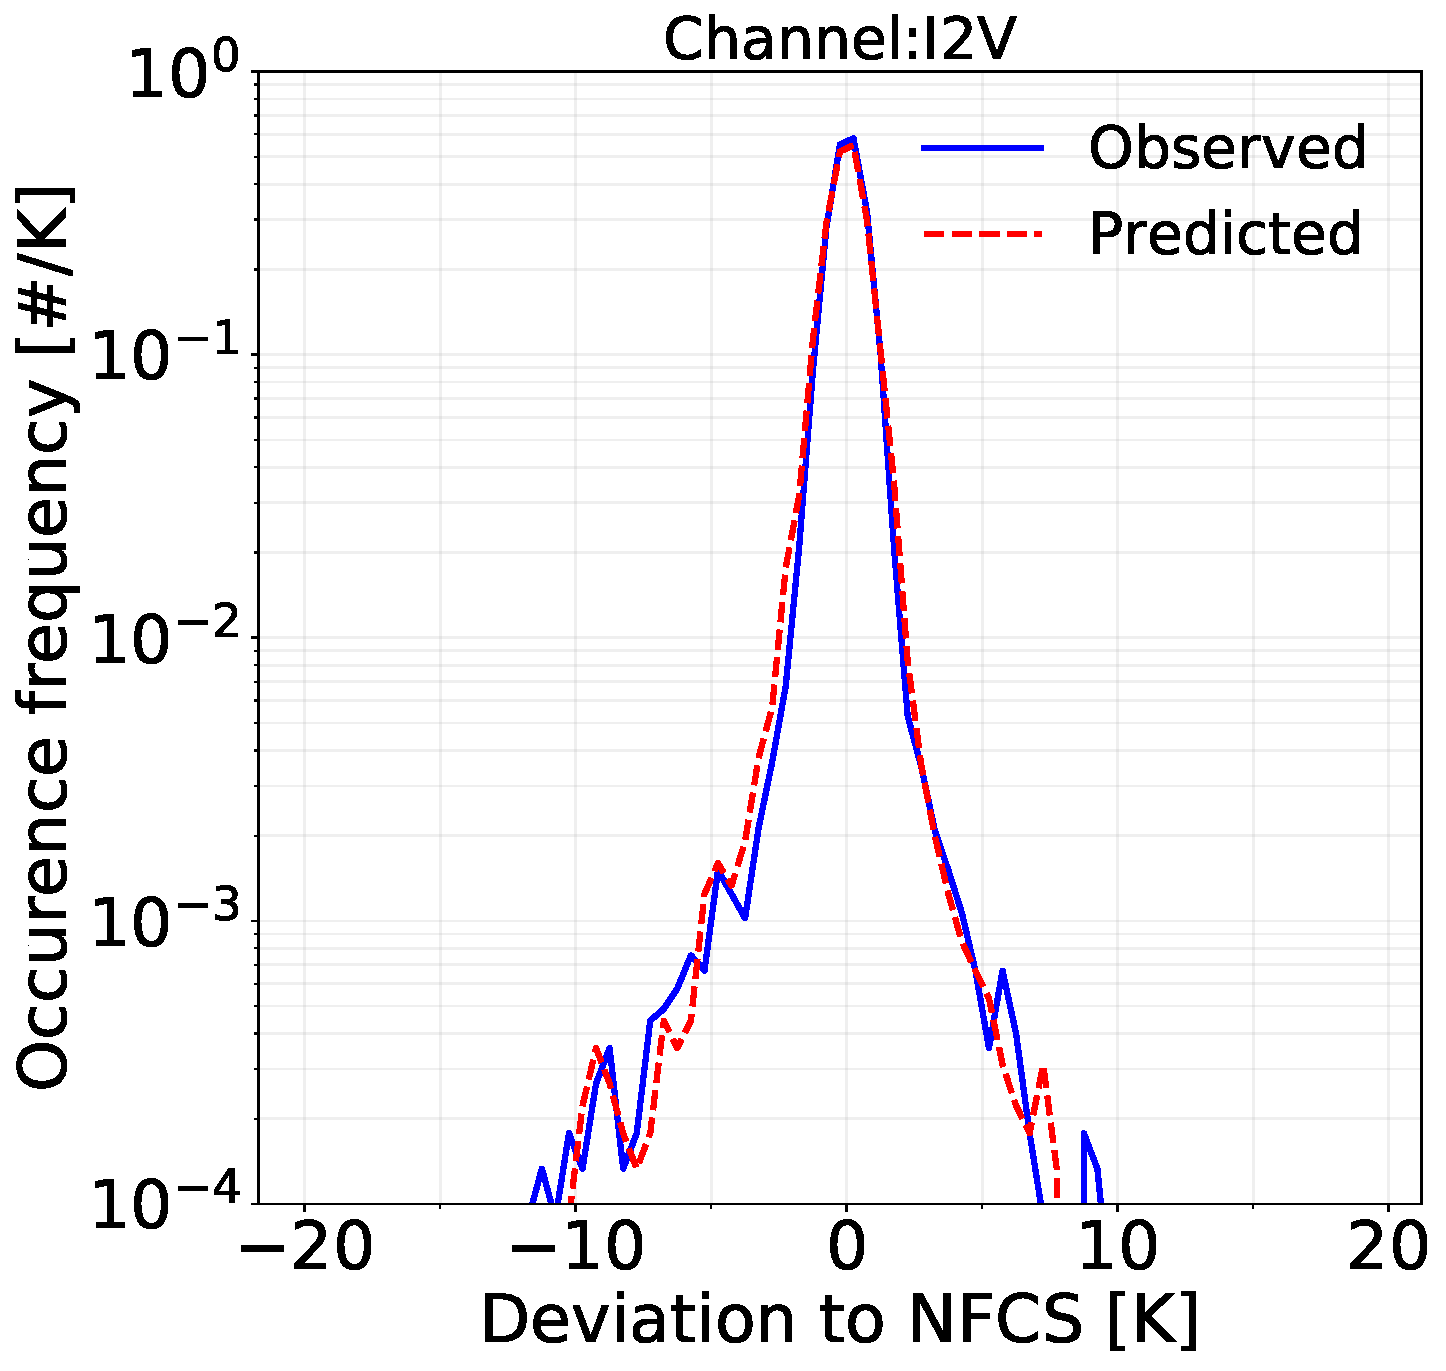
\includegraphics[width=150mm]{Figures/deviation_posterior_samples_I2V.pdf}	
	\caption{The distribution of predicted errors and observed errors for I2V as obtained from QRNN-single and QRNN-all for the test dataset. The predicted errors are estimated as deviation of random samples from posteriori distribution to corresponding median values.}
	\label{fig:predicted_errors}	
\end{figure*}
\begin{figure}[t]
	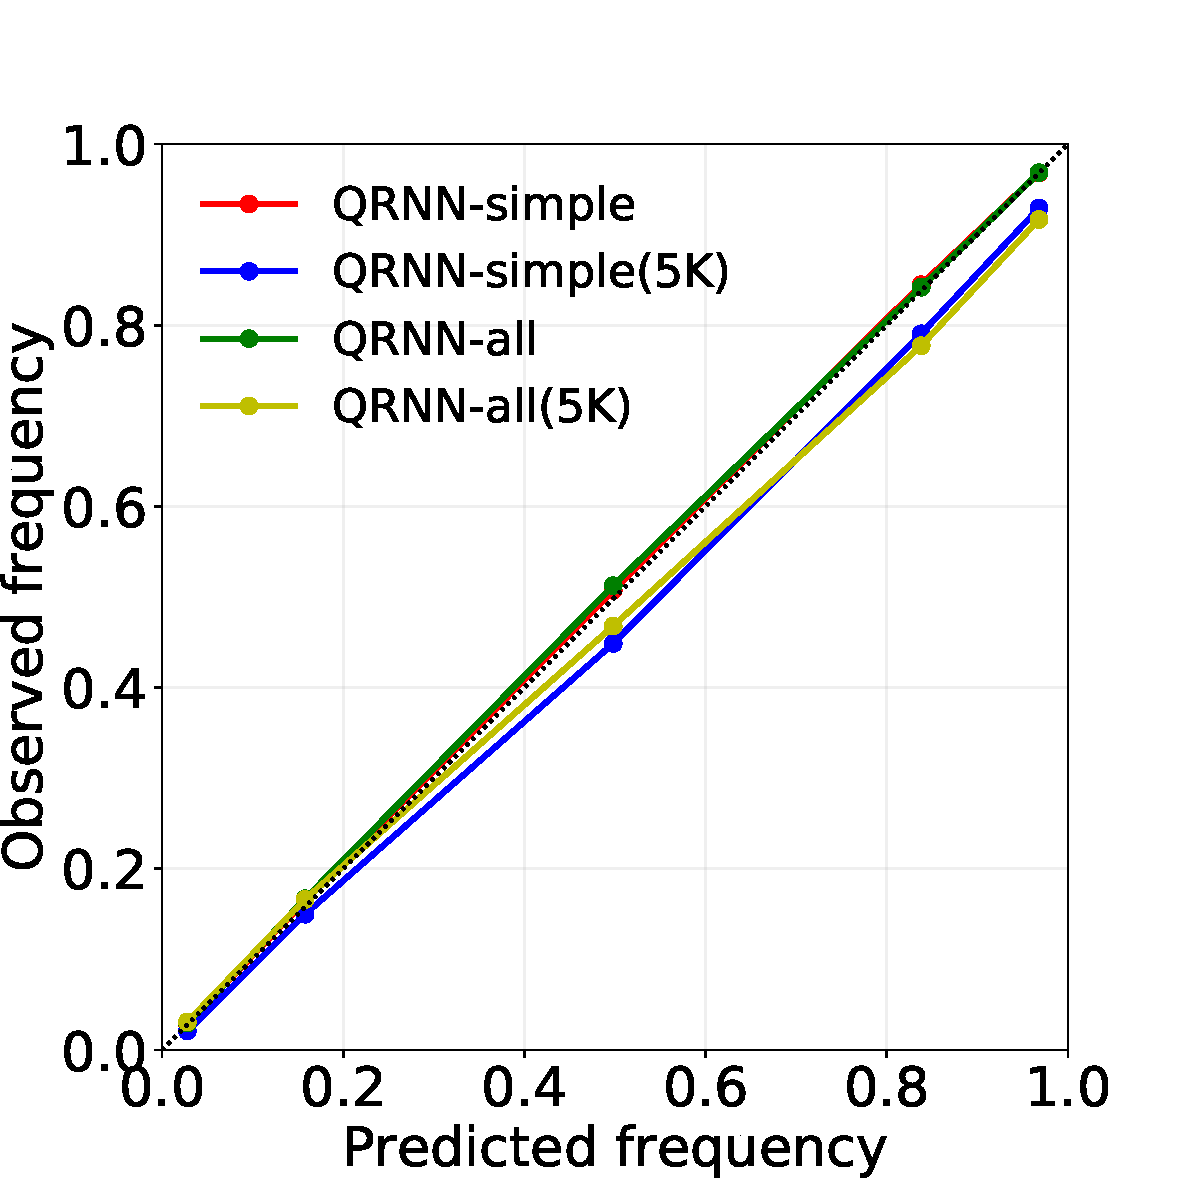
\includegraphics[height = 70mm]{Figures/calibration_QRNN_I1V.pdf}	
	\caption{Calibration of the prediction intervals obtained from QRNN-single and QRNN-all for I1V. }
	\label{fig:calibration_I1V}	
\end{figure}
\begin{figure*}[t]
	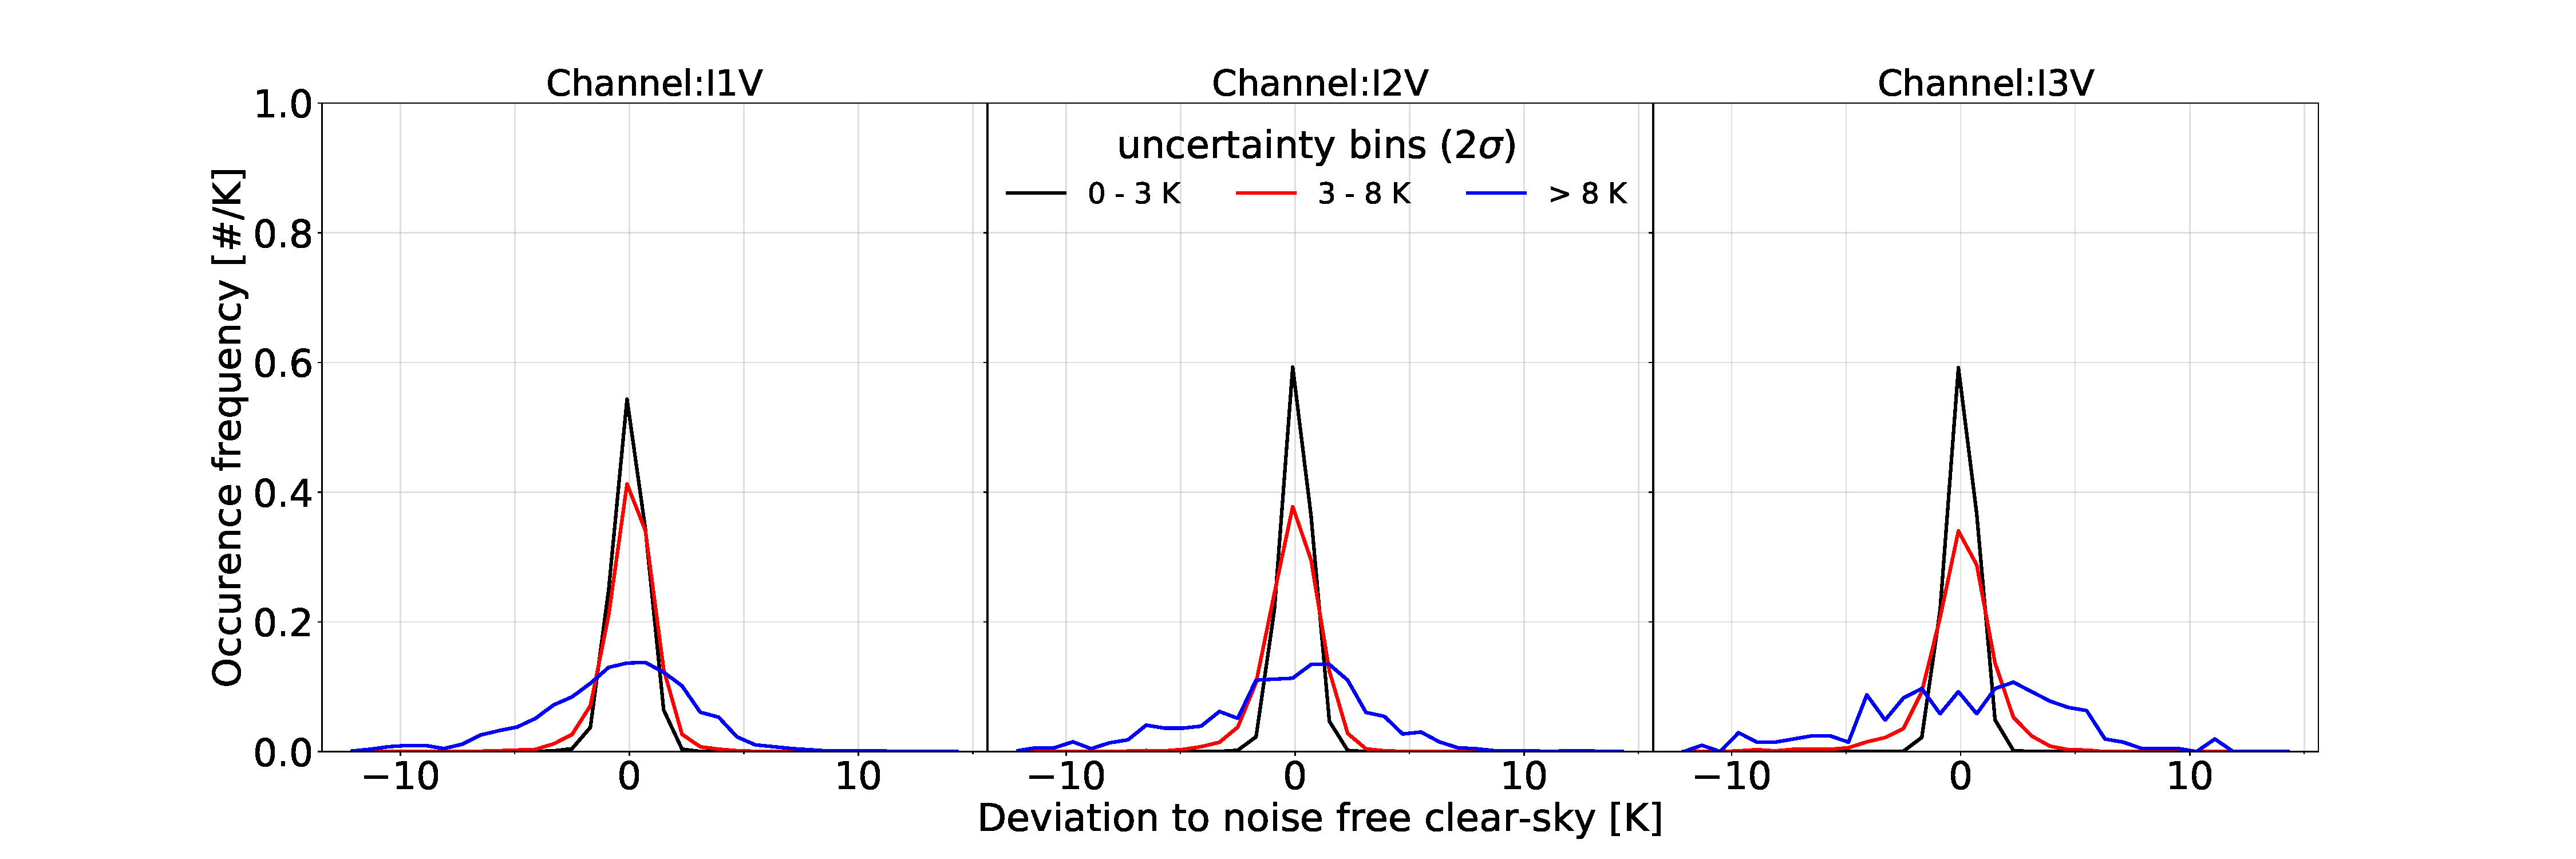
\includegraphics[width=\textwidth]{Figures/PDF_uncertainty_bins_QRNN-single.pdf}	
	\caption{Distribution of errors binned according to their uncertainty. Results are from QRNN-single for channels I1V, I2V and I3V.}
	\label{fig:error_distribution_uncertainty_bins}	
\end{figure*}

The biggest advantage of using QRNN is estimation of case-specific uncertainties. The quantiles can be used to construct a probability distribution of the predictions in contrast to other correction approaches which give out only point estimates. 

In order to analyse the prediction uncertainty, the deviations of predicted quantiles from its median value are estimated. Fig.~\ref{fig:prediction_uncertainty_I2V} shows the spread of prediction uncertainties over different quantiles for randomly chosen 1500 cases. The large spread in the predicted errors indicates that QRNN is successful in representing uncertainties for each case individually, rather than expressing them as a single measure for all cases. In the latter case, the uncertainty estimates would be concentrated along a narrow interval. Among the cases associated with low uncertainty, the distribution is quite symmetric along the median value. These cases are concentrated along a narrow interval and lie close to the black curve representing a Gaussian spread. On the contrast, cases with high uncertainty are unequally spaced and have a larger spread over positive quantiles than negative quantiles. Thus QRNN is capable of capturing non-Gaussian  error distributions as well. 

Fig.~\ref{fig:predicted_errors} shows the comparison of observed errors (prediction accuracy) to predicted errors. The predicted dataset is constructed by drawing random samples from the posteriori distribution. We do not derive any sample from outside $\pm3\sigma$.  The predicted error is deviation of random sample to its median. For QRNN-single, the predicted and observed errors have good agreement for the peak of the distribution, but the predicted errors are spread out asymmetrically. For QRNN-all, the predicted and observed errors have a better agreement and the spread is symmetric for the former. The results show that both QRNN-single and QRNN-all are not able to represent the left wings of the distribution. This could also be a sampling issue, as the high errors we try to predict constitute a very small part of the complete dataset.  

For further analysis, we compared the distribution of predictions from QRNN with the a priori distribution. In a  high performing QRNN model, the posteriori distribution of the predictions should be similar to the a priori distribution of training dataset. A straightforward way to compare the two distribution is to plot the frequency of predictions and frequency of the true value in different prediction intervals. This is also commonly known as calibration plot. Fig.~\ref{fig:calibration_I1V} shows the calibration of the prediction intervals on the test dataset for I1V. For both QRNN models, the predictions for the complete test dataset are well calibrated and follow the y=x line. This shows that the training and test datasets come from the same a priori distribution. On the other hand, when only the cases with  cloud correction greater than 10\,K are considered, for both models, the predictions in all the intervals are poorly calibrated. In this case the calibration curve lies below the y=x line, indicating that the predicted intervals are too narrow, or the uncertainty is underestimated. The clear-sky cases dominate the test/training dataset, thus the a priori distribution is representative of the same. The a priori distribution of cloudy cases is different to the clear-sky cases, therefore the predictions are poorly calibrated for the former. We also plotted the calibration curves for I2V and I3V (figure not shown). For both these channels, predictions over complete dataset were well calibrated for both QRNN-single and QRNN-all, but for subset with threshold 10\,K, slightly poor calibrations were observed in QRNN-single. This is in contrast with I1V, where both models had poor calibrations for cases with high cloud impact. 

Lastly, we investigated that if the uncertainty estimates given by QRNN are representative of prediction accuracy. Fig.~\ref{fig:error_distribution_uncertainty_bins} shows the errors of best estimate binned by their corresponding uncertainty in $\pm2\sigma$  confidence interval. Similar results were also obtained for QRNN-all (figure not shown). For all three channels, the spread of error distribution increases as the uncertainty about the accuracy of the trial increases. The cases with high certainty have a narrow and sharp distribution, and the errors are mostly less than $\pm$2.5\,K. With increase in the uncertainty, frequency of cases with high accuracy decreases and the distributions spread out symmetrically to higher errors. Poor predictions occur more frequently when uncertainty is high. Cases with accurate predictions yet high uncertainty are also present. In spite of individual variations in the error distributions for each channel, predictions and their corresponding uncertainties followed the same relationship.

The results show that both QRNN-single and QRNN-all are successful in providing well calibrated probabilistic predictions of the posterior distributions except for few cases associated with high cloud impact. This is not unexpected as such cases form a small subset of the training set and their priori distribution is different from the entire dataset. Since such cases form only a fraction of the training dataset, it can be hard to train the model to predict them accurately. A larger training dataset would be required to increase the representation of such cases in QRNN.

\subsection{MWI}
%
In this section, we discuss results when all 183\,GHz MWI channels are used for ``self'' cloud filtering/correction (QRNN-mwi). We also describe the performance of QRNN when sub-mm channels from ICI are used to train MWI channels.
\subsubsection{MWI alone}
%
%t
\begin{table*}[t]
	\caption{Error statistics for predictions from QRNN-mwi. The labels Filtered(7.5\,K), Predicted(All) and Predicted(7.5\,K) are same as described in Table~\ref{tab:error_statistics_ici}}
	\label{tab:statistics_mwi-alone}
	\begin{tabular}{llrr|rrr}
		\tophline
		&&\multicolumn{2}{c|}{Simulations}& \multicolumn{3}{c}{QRNN-single} \\
		\cline{3-7}
		%		\hline
		&&   Clear-sky &   All-sky &  Filtered(7.5\,K) & Predicted & Predicted(7.5\,K) \\
		\middlehline
		MWI-14 		&bias     & -0.00 & -1.86 & -0.50(4.06\%) & -0.14 & -0.12 \\
					&mae      &  0.96 &  2.58 &  1.25 &  1.12 &  1.00 \\
					&std      &  1.20 &  9.00 &  1.94 &  1.86 &  1.52 \\
					&skewness &  0.01 & -8.20 & -3.03 & -0.88 & -2.15 \\ 
		\middlehline
		MWI-15 		&bias     & 0.01 & -1.23 & -0.40(2.84\%) & -0.13 & -0.11 \\
					&mae      & 0.95 &  1.99 &  1.18 &  0.74 &  0.66 \\
					&std      & 1.20 &  6.55 &  1.73 &  1.32 &  1.11 \\
					&skewness & 0.01 & -9.67 & -2.34 & -2.44 & -2.89 \\
		\middlehline	
		MWI-16 		&bias     & 0.00 &  -0.85 & -0.29(1.94\%) & -0.12 & -0.10 \\
					&mae      & 0.96 &   1.64 &  1.10 &  0.68 &  0.63 \\
					&std      & 1.20 &   5.39 &  1.54 &  1.15 &  0.96 \\
					&skewness & 0.00 & -11.62 & -1.97 & -3.71 & -3.22 \\	
		\middlehline			
		MWI-17 		&bias     & -0.00 &  -1.04 & -0.32(2.41\%) & -0.13 & -0.11 \\
					&mae      &  0.96 &   1.83 &  1.12 &  0.73 &  0.67 \\
					&std      &  1.20 &   6.29 &  1.59 &  1.21 &  1.02 \\
					&skewness & -0.01 & -10.69 & -2.13 & -3.45 & -3.23 \\	
		\middlehline			
		MWI-18 		&bias     &  0.01 &  -0.66 & -0.26(1.37\%) & -0.12 & -0.10 \\
					&mae      &  0.96 &   1.47 &  1.08 &  0.80 &  0.76 \\
					&std      &  1.20 &   4.66 &  1.51 &  1.23 &  1.08 \\
					&skewness & -0.00 & -12.80 & -2.03 & -2.99 & -2.25 \\	
		\bottomhline				
	\end{tabular}	
	\belowtable{} % Table Footnotes
\end{table*}
\begin{figure}[t]
	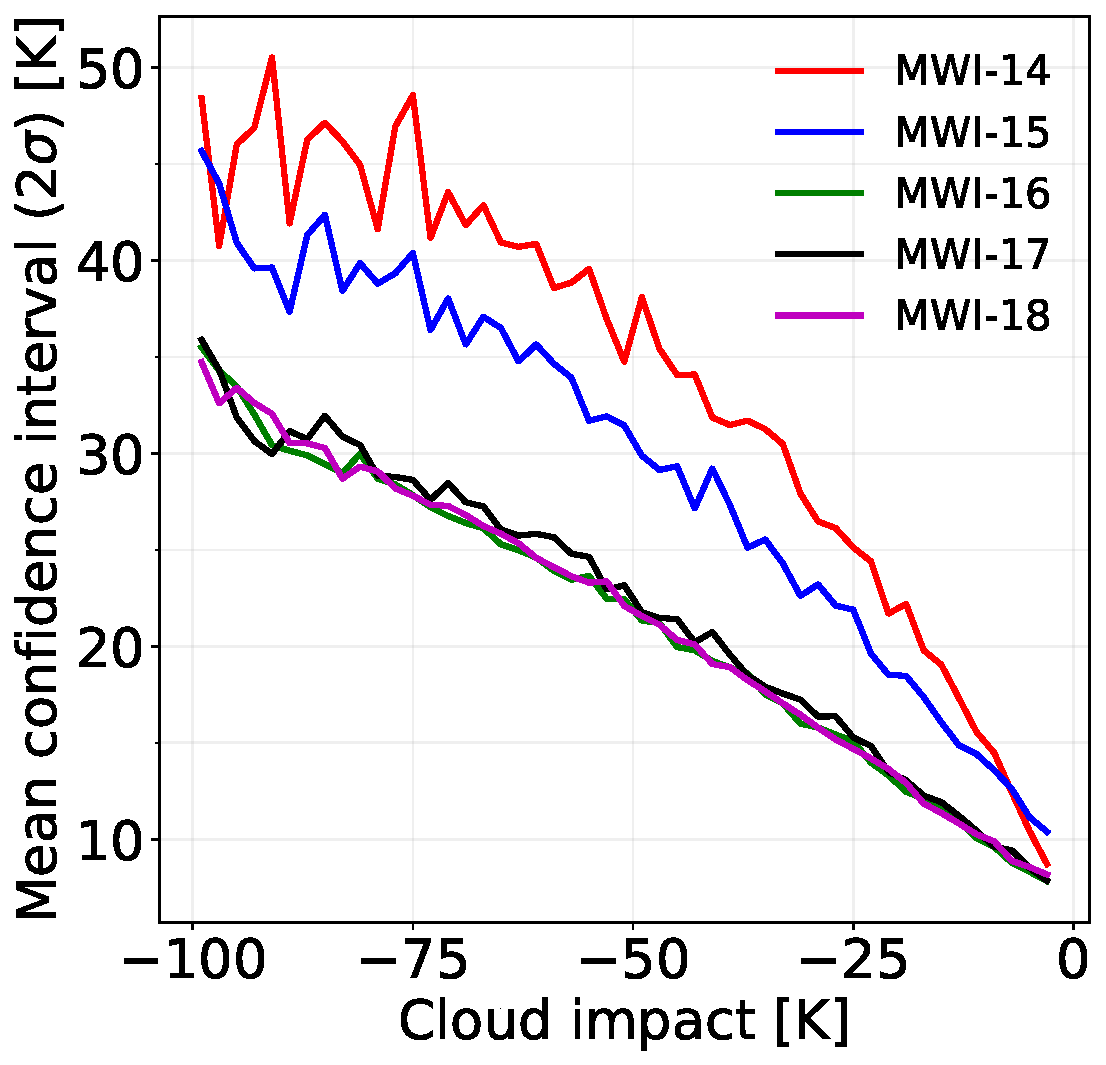
\includegraphics[width = 70mm]{Figures/cloud_impact_uncertainty_MWI.pdf}	
	\caption{The average confidence intervals (2$\sigma$) plotted against the magnitude of cloud impact for all MWI channels.}
	\label{fig:uncertainty_cloud_impact}	
\end{figure}
QRNN-mwi is designed to provide basis for a cloud correction approach applicable to current satellites, which lack the higher frequency channels. 

Table~\ref{tab:statistics_mwi-alone} shows the results for all 183\,GHz channels of MWI. MWI channels have a higher measurement uncertainty than ICI, so a higher filtering threshold is selected. All cases with cloud correction greater than 7.5\,K are considered as cloudy and filtered out. With pure-filtering, only 4\% of the cases are filtered out for MWI-14, but the bias reduces from -1.86\,K to -0.50\,K. For the predictions, the average bias is -0.14\,K. For both filtering and correction, a significant reduction in the errors is observed but the resulting values are still high and indicate only partial success of the method. For other channels also, a similar performance is observed.  For MWI-15, cloud correction reduces the average error from -1.23\,K to -0.13\,K  and the corresponding decrease in standard deviation is 6.55\,K to 1.32\,K. Filtering the predicted cases improves the bias and standard deviation further by 15\%. Interestingly, even with partial correction, the standard deviation is lower than the measurement noise. For MWI-16, the bias for predictions is -0.12\,K compared to -0.85\,K for the measurements. The corresponding standard deviation is  1.15\,K, which is again smaller than the measurement noise(1.20\,K). MWI-17 also has a similar performance. MWI-18 is least affected by cloud impact among the five channels. The average deviation of the measurement data to NFCS values is only -0.66\,K which reduces to -0.12\,K with QRNN. After filtering 1.37\% cases with high cloud impact, only a slight improvement in the accuracy is observed but the variability of errors decreases from 1.23\,K to 1.08\,K. The results show that QRNN-mwi is partially successful in removing the cloud impact. A significant reduction in the deviation to NFCS values indicates that though most cases with high cloud impact can be removed/corrected, the cases with residual cloud impact and uncorrected cases deteriorate the performance. Using a low threshold filter can improve the accuracy, but at the cost of excessive removal of clear-sky cases. 

The five frequencies are sensitive to different regions of the troposphere so not all clouds are equally represented in all. The brightness temperature of same cloud measured at different frequencies can be valuable to train QRNN. However the hydrometeor impact from regions where the weighting functions match poorly cannot be represented adequately in QRNN. As a consequence, the predictions are poor. In constrast, the clear-sky measurements of the same scene from multiple channels, reinforces the QRNN predictions. The measurement noise in all channels is stationary and uncorrelated, thus the predictions benefit from the additional information, and averaging cancels out the noise component. As clear-sky cases occur more frequently, the effect is quite prominent.

Further, we investigate if uncertainty estimates from QRNN-mwi are representative of prediction errors. Fig.~\ref{fig:uncertainty_cloud_impact} displays the average predicted errors in 94\% confidence interval, for different cloud impacts. For all five channels, the predictions with small or relatively low cloud signal have a low uncertainty or in other words have high sharpness. As fraction of cloud impact increases, the predictions become increasingly uncertain. Most uncertain predictions occur for the outermost channels (MWI-14, MWI-15). These channels also have the lowest prediction accuracy.  Thus, the QRNN predictions possess a multivariate representation of uncertainty. The uncertainty of cases with varying cloud impacts can be expressed individually.

\subsubsection{MWI and ICI}
%t
\begin{table*}[t]
	\caption{Same as Table~\ref{tab:error_statistics_ici}, but for channels MWI-15 and MWI-16. Results are from QRNN-single.}
	\label{tab:statistics_mwi}
	\begin{tabular}{llrr|rrr}
		\tophline
				&&\multicolumn{2}{c|}{Simulations}& \multicolumn{3}{c}{QRNN-single} \\
				\cline{3-7}
				%		\hline
				&&   Clear-sky &   All-sky &  Filtered(5\,K) & Predicted & Predicted(5\,K) \\
		\middlehline
		MWI-15  &Bias     &  0.00 & -1.23 & -0.26 & -0.04 & -0.03 \\
				&MAE      &  0.64 &  1.70 &  0.76 &  0.56 &  0.50 \\
				&STD      &  0.81 &  6.48 &  1.01 &  0.86 &  0.64 \\
				&Skewness & -0.00 & -9.97 & -1.15 & -1.78 & -0.15 \\
		\middlehline
		MWI-16  &Bias     & 0.00 &  -0.85 & -0.22 & -0.06 & -0.05 \\
				&MAE      & 0.64 &   1.34 &  0.73 &  0.55 &  0.50 \\
				&STD      & 0.80 &   5.31 &  0.96 &  0.83 &  0.63 \\
				&Skewness & 0.01 & -12.08 & -1.02 & -2.25 & -0.11 \\
		\bottomhline			
	\end{tabular}	
	\belowtable{} % Table Footnotes
\end{table*}
In this section, we combine the measurements from MWI-15(MWI-16) and the ICI sub-mm channels to predict MWI-15(MWI-16). Since we assume that all channels are remapped to a common footprint, channels MWI-14, MWI-17 and MWI-18 are virtually identical to I1V, I2V and I3V, and results for them are not shown separately.

Table~\ref{tab:statistics_mwi} shows the error metrics of NFCS predictions from simulations. For MWI-15, the average deviations of measurements from NFCS values is -1.23\,K, and the MAE is 1.70\,K. When all cases are corrected, the resulting average bias is -0.04\,K and the MAE reduces to 0.56\,K. If only pure-filtering is made, the average bias is -0.26\,K and MAE is 0.76\,K, suggesting that a significant number of cases with non-zero cloud impact pass through. As seen for ICI, best results are obtained  when filtering is made on the corrected dataset. Similar accuracy is seen for MWI-16, although it has slightly lower cloud impact. 

These results show that even though ICI and MWI are two different instruments, their channels can benefit from each other. Although re-mapping to a common footprint would slighly compromise the data quality, a high accuracy achieved with simulations suggests that the QRNN would work well when actual measurements are available.

\subsection{AWS}
%
%t
\begin{table*}[t]
	\caption{Same as Table~\ref{tab:error_statistics_ici}, but for channels AWS channels. Results are from QRNN-single. }
	\label{tab:statistics_qrnn_aws}
	\begin{tabular}{llrr|rrr}
		\tophline
		&&\multicolumn{2}{c|}{Simulations}& \multicolumn{3}{c}{QRNN-single} \\
		\cline{3-7}
		%		\hline
		&&   Clear-sky &   All-sky &  Filtered(5\,K) & Predicted & Predicted(5\,K) \\
		\middlehline
		AWS-32  &bias     & 0.00 & -1.32 & -0.26 & -0.03 & -0.02 \\
				&mae      & 0.36 &  1.57 &  0.52 &  0.54 &  0.43 \\
				&std      & 0.46 &  6.42 &  0.85 &  1.02 &  0.61 \\
				&skewness & 0.01 & -8.43 & -3.65 & -0.07 & -1.98 \\
		\middlehline
		AWS-33	&Bias     & -0.01 & -0.98 & -0.25 & 0.02 &  0.01 \\
				&MAE      &  0.36 &  1.23 &  0.51 & 0.49 &  0.42 \\
				&STD      &  0.45 &  4.70 &  0.80 & 0.76 &  0.56 \\
				&skewness & -0.00 & -8.78 & -2.92 & 0.04 & -0.79 \\
		
		\middlehline
		AWS-34	&Bias     &  0.00 &  -0.68 & -0.20 &  0.02 &  0.01 \\
				&MAE      &  0.51 &   1.07 &  0.61 &  0.51 &  0.46 \\
				&STD      &  0.64 &   3.67 &  0.84 &  0.75 &  0.60 \\
				&skewness & -0.00 & -10.32 & -1.70 & -0.55 & -0.59 \\
		\middlehline
		AWS-35	&Bias     &  0.00 &  -0.43 & -0.15 & 0.01 &  0.00 \\
				&MAE      &  0.50 &   0.84 &  0.57 & 0.48 &  0.44 \\
				&STD      &  0.63 &   2.65 &  0.77 & 0.71 &  0.57 \\
				&skewness & -0.01 & -12.49 & -1.34 & 0.40 & -0.29 \\
		\middlehline
		AWS-36  &Bias     & 0.00 &  -0.28 & -0.11 &  0.03 &  0.03 \\
				&MAE      & 0.70 &   0.90 &  0.74 &  0.63 &  0.60 \\
				&STD      & 0.88 &   2.06 &  0.96 &  0.86 &  0.76 \\
				&skewness & 0.01 & -11.80 & -0.53 & -0.35 & -0.20 \\
		\bottomhline				
	\end{tabular}
	\belowtable{} % Table Footnotes
\end{table*}
%f
%\begin{figure}[t]
%	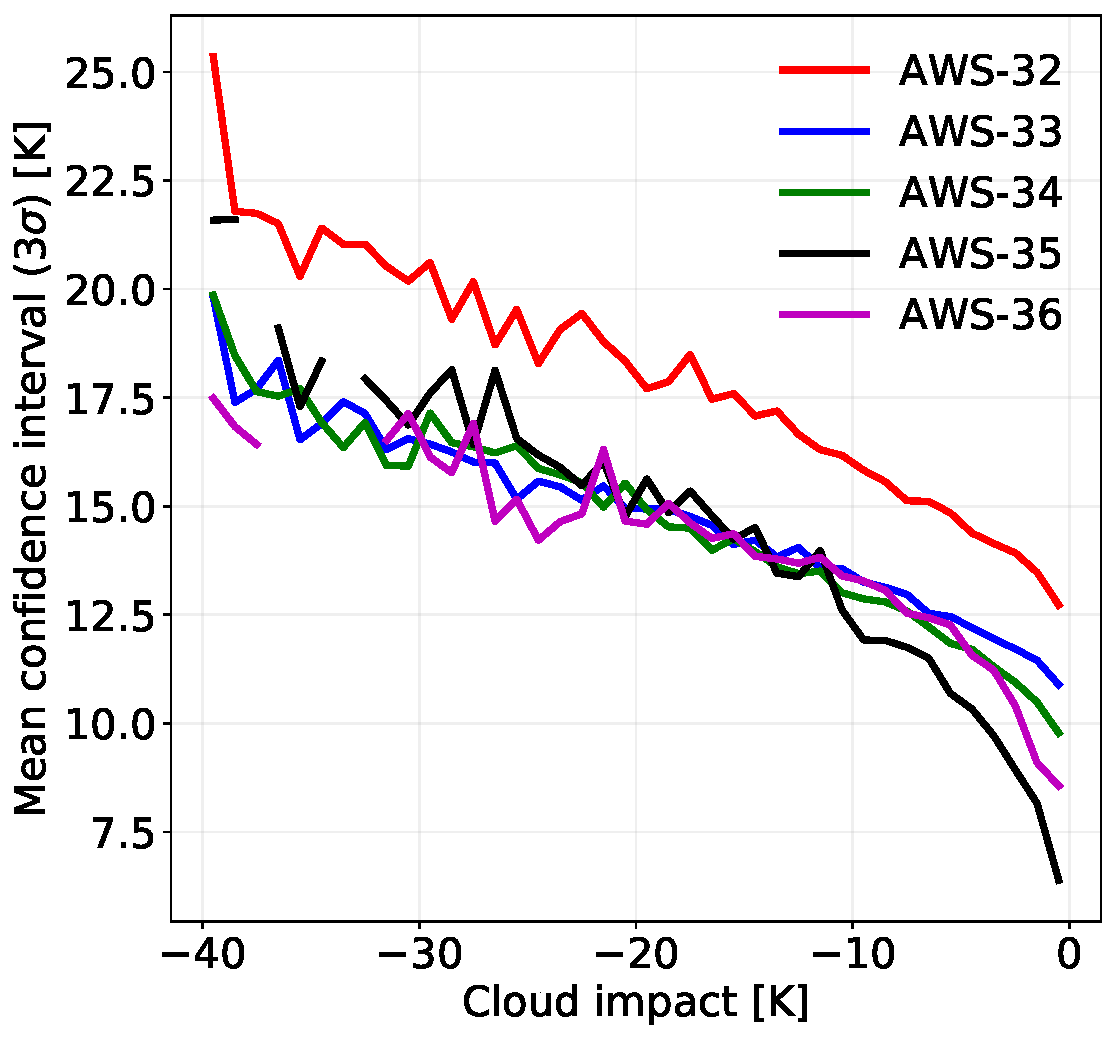
\includegraphics[width = 80mm]{Figures/cloud_impact_uncertainty_AWS.pdf}	
%	\caption{The average confidence intervals (2$\sigma$) plotted against the magnitude of cloud impact for all AWS channels.}
%	\label{fig:uncertainty_cloud_impact}	
%\end{figure}

In this section, we investigate the possibility of using only channels around 325\,GHz for cloud correction at 183\,GHz. This special case of utilising only 325\,GHz channel can be relevant for smaller satellite missions like AWS where higher sub-mm channels are not available. 

In an analogy between the results from ICI channels, we perform a similar error distribution analysis 
and the results are displayed in Table~\ref{tab:statistics_qrnn_aws}. For channel AWS-32, the average bias and standard deviation in the prediction errors is -1.34\,K and 5.91\,K respectively. However, after correction, the bias and standard deviation are -0.08\,K and 1.0\,K. A decrease in the skewness of error distributions is evident, but a relatively high values after prediction indicate presence of cases with partially-corrected cloud impact. For AWS-33, the predictions have slightly higher accuracy than AWS-32. The MAE in predictions is only 0.50\,K in comparison to 1.23\,K for the measurements. Similar results are also seen for AWS-35 and AWS-36. For both channels, the error distributions are relatively more symmetric than the other channels. Also, it is worth to noting that when cases with 5\,K cloud correction are removed, the spread of prediction errors is narrower than noise. 

Overall the results demonstrate that QRNN is successful in predicting the NFCS data for AWS-33, AWS-34, AWS-35 and AWS-36 and partially for AWS-32. The prediction error distributions are symmetric with low bias and standard deviation. The cases with high error are mostly associated with high cloud impact and constitute only a small fraction of the total dataset. Excluding such cases decreases the errors and in fact the spread of errors for AWS-34, AWS-35 and AWS-36 is smaller than noise. Removal of cases with high cloud impact, increases the representation of cases in cloud-free conditions, and for such cases, QRNN predictions can be seen as a weighted mean between the two channels. For AWS-32, QRNN is only partially successful in reducing the impact of hydrometeors. The prediction errors have significantly lower spread than the measurements, but cases with partially corrected cloud impact deteriorates the overall accuracy. Since 325\,GHz cannot provide a full coverage for hydrometeor impact in AWS-32, the testing data will inevitably contain cases for which QRNN has not trained for. Prediction for such cases would be inaccurate and highly uncertain. In such cases, the predictions should be used with caution. 

%In order to analyse the performance of QRNN with respect to uncertainty, the interrelation between the uncertainty estimates and cloud impact was investigated. Fig~\ref{fig:uncertainty_cloud_impact} displays the plot between mean uncertainty estimates for $2\sigma$ confidence interval and the cloud impact. For all five channels, the predictions with small or relatively low cloud signal have a low uncertainty or in other words have high sharpness. As fraction of cloud impact increases, the predictions become increasingly uncertain. However, this does not imply that the prediction accuracy is low. 


\section{Conclusion and outlook}  %% \conclusions[modified heading if necessary]
%
To be written \dots




%% The following commands are for the statements about the availability of data sets and/or software code corresponding to the manuscript.
%% It is strongly recommended to make use of these sections in case data sets and/or software code have been part of your research the article is based on.

\codeavailability{TEXT} %% use this section when having only software code available


\dataavailability{TEXT} %% use this section when having only data sets available


\codedataavailability{TEXT} %% use this section when having data sets and software code available


\sampleavailability{TEXT} %% use this section when having geoscientific samples available


\videosupplement{TEXT} %% use this section when having video supplements available


\appendix
\section{}    %% Appendix A

\subsection{}     %% Appendix A1, A2, etc.


\noappendix       %% use this to mark the end of the appendix section. Otherwise the figures might be numbered incorrectly (e.g. 10 instead of 1).

%% Regarding figures and tables in appendices, the following two options are possible depending on your general handling of figures and tables in the manuscript environment:

%% Option 1: If you sorted all figures and tables into the sections of the text, please also sort the appendix figures and appendix tables into the respective appendix sections.
%% They will be correctly named automatically.

%% Option 2: If you put all figures after the reference list, please insert appendix tables and figures after the normal tables and figures.
%% To rename them correctly to A1, A2, etc., please add the following commands in front of them:

\appendixfigures  %% needs to be added in front of appendix figures

\appendixtables   %% needs to be added in front of appendix tables

%% Please add \clearpage between each table and/or figure. Further guidelines on figures and tables can be found below.



\authorcontribution{TEXT} %% this section is mandatory

\competinginterests{TEXT} %% this section is mandatory even if you declare that no competing interests are present

\disclaimer{TEXT} %% optional section

\begin{acknowledgements}
TEXT
\end{acknowledgements}




%% REFERENCES


 \bibliographystyle{copernicus}
 \bibliography{references.bib}

\end{document}
